% -*- latex -*-


\chapter{Strategies}
\label{chap:Strategies}

\index{strategy|(}

\IceT contains several parallel image compositing algorithms.  The type of
compositing algorithm to use is selected by choosing a
\index{strategy}\keyterm{strategy}.  This chapter describes the underlying
algorithm of each strategy.  This user's guide will give qualitative
comparisons between the strategies, but for a more quantitative analysis,
see the following paper.

\begin{quote}
  Kenneth Moreland, Brian Wylie, and Constantine Pavlakos.  ``Sort-last
  parallel rendering for viewing extremely large data sets on tile
  displays,'' In \emph{Proceedings of IEEE Symposium on Parallel and
    Large-Data Visualization and Graphics}, October 2001, pp. 85--154.
\end{quote}

A strategy is specified using the \CFunc{icetStrategy} function.

\begin{Table}{3}
  \textC{void }\CFunc{icetStrategy}\textC{(}&\textC{IceTEnum}&\CArg{strategy}\quad\textC{);}
\end{Table}

The \CArg{strategy} is set to one of the following identifiers.

% -*- latex -*-

  \begin{Description}
  \item[\CEnum{ICET\_STRATEGY\_SEQUENTIAL}]
    Basically applies a ``traditional'' single tile composition (such as
    binary swap) to each tile in the order they were defined.  Because each
    process must take part in the composition of each tile regardless of
    whether they draw into it, this strategy is usually inefficient when
    compositing for more than one tile, but is recommended for the single
    tile case because it bypasses some of the communication necessary for
    the other multi-tile strategies.
    \index{strategy!sequential}
  \item[\CEnum{ICET\_STRATEGY\_DIRECT}] As each process renders an image
    for a tile, that image is sent directly to the process that will
    display that tile.  This usually results in a few processes receiving
    and processing the majority of the data, and is therefore usually an
    inefficient strategy.
    \index{strategy!direct}
  \item[\CEnum{ICET\_STRATEGY\_SPLIT}] Like \CEnum{ICET\_STRATEGY\_DIRECT},
    except that the tiles are split up, and each process is assigned a
    piece of a tile in such a way that each process receives and handles
    about the same amount of data.  This strategy is often very efficient,
    but due to the large amount of messages passed, it has not proven to be
    very scalable or robust.
    \index{strategy!split}
  \item[\CEnum{ICET\_STRATEGY\_REDUCE}] A two phase algorithm.  In the
    first phase, tile images are redistributed such that each process has
    one image for one tile.  In the second phase, a ``traditional'' single
    tile composition is performed for each tile.  Since each process
    contains an image for only one tile, all these compositions may happen
    simultaneously.  This is a well rounded strategy that seems to perform
    well in a wide variety of multi-tile applications.  (However, in the
    special case where only one tile is defined, the sequential strategy is
    probably better.)
    \index{strategy!reduce}
  \item[\CEnum{ICET\_STRATEGY\_VTREE}] An extension to the binary tree
    algorithm for image composition.  Sets up a ``virtual'' composition
    tree for each tile image.  Processes that belong to multiple trees
    (because they render to more than one tile) are allowed to float
    between trees.  This strategy is not quite as well load balanced as
    \CEnum{ICET\_STRATEGY\_REDUCE} or \CEnum{ICET\_STRATEGY\_SPLIT}, but
    has very well behaved network communication.
    \index{strategy!virtual~trees}
  \end{Description}


A string documenting the current strategy can be retrieved with the
\CFunc{icetGetStrategyName} function.  The following sections describe the
strategies in more detail.

To describe the \IceT compositing algorithms, we will use the example
parallel rendering problem shown in Figure~\ref{fig:ExampleInputs} where 6
processes are each rendering their own piece of a shuttle model to a two
tile display.

\begin{figure}
  \centering
  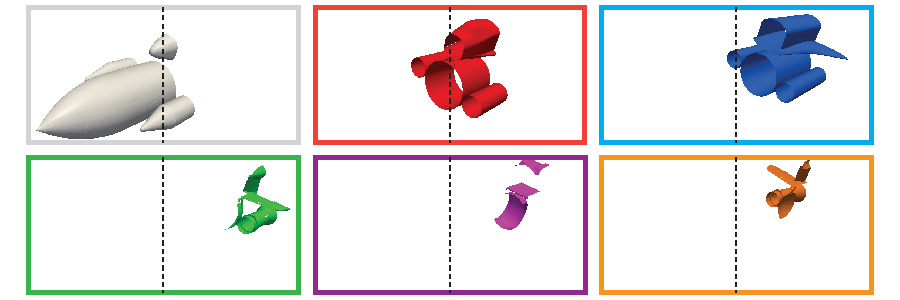
\includegraphics{images/AllInput}
  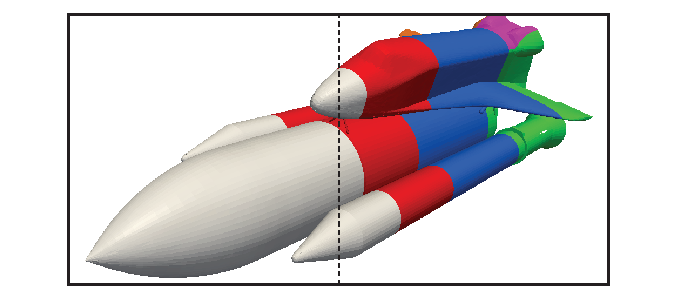
\includegraphics{images/CompositedInput}
  \caption[Example compositing problem.]{An example of six processes
    rendering to two tiles (top) and their composited image (bottom).}
  \label{fig:ExampleInputs}
\end{figure}

In this example, processes are denoted, in no particular order, by the
colors gray, red, blue, green, purple, and orange.  The colors of the
geometry correspond to the process that generated each piece.  Image
boarder colors denote the process that generates and holds that image.
(Apologies to those having troubles resolving the colors due to poor
display, printout, or vision deficiencies.  It should not be hard to follow the
descriptions either way.)

\section{Single Image Compositing}
\label{sec:Strategies:SingleImageCompositing}

\index{single~image~composite|(}
\index{compositing!single~image|(}

Before discussing the multi-tile image compositing algorithms implemented
by \IceT, we visit the standard single image compositing algorithms.  You
cannot directly use a single image compositing algorithm as a strategy
(most of the multi-tile algorithms work well in ``single-tile'' mode), but
these compositing algorithms are used as ``subroutines'' in some of the
multi-tile algorithms.  A reference to a
\index{single~image~composite~network}\keyterm{single image composite
  network} in the subsequent compositing algorithm descriptions refers to
the algorithms described here.

You can, however, choose which single image strategy is used by the main
multi-tile strategy.  This is selected with the
\CFunc{icetSingleImageStrategy} function.

\begin{Table}{3}
  \textC{void }\CFunc{icetSingleImageStrategy}\textC{(}&\textC{IceTEnum}&\CArg{strategy}\quad\textC{);}
\end{Table}

The \CArg{strategy} is set to one of the following enumerations.

% -*- latex -*-

\begin{Description}
\item[\CEnum{ICET\_SINGLE\_IMAGE\_STRATEGY\_AUTOMATIC}] Automatically
  chooses which single image strategy to use based on the number of
  processes participating in the composition.
  \index{single~image~strategy!automatic}
\item[\CEnum{ICET\_SINGLE\_IMAGE\_STRATEGY\_BSWAP}] The classic binary swap
  compositing algorithm.  At each phase of the algorithm, each process
  partners with another, sends half of its image to its partner, and
  receives the opposite half from its partner.  The processes are then
  partitioned into two groups that each have the same image part, and the
  algorithm recurses.
  \index{single~image~strategy!binary~swap}
\item[\CEnum{ICET\_SINGLE\_IMAGE\_STRATEGY\_TREE}] At each phase, each
  process partners with another, and one of the processes sends its entire
  image to the other.  The algorithm recurses with the group of processes
  that received images until only one process has an image.
  \index{single~image~strategy!tree}
\end{Description}


A string documenting the current strategy can be retrieved with the
\CFunc{icetGetSingleImageStrategyName} function.  The following sections
describe the single image strategies in more detail.

\subsection{Tree Compositing}

\index{compositing!tree|(}
\index{tree~composite|(}
\index{binary~tree~composite|(}

The \keyterm{tree composite} algorithm (sometimes also called binary tree
composite due to its pair-wise grouping) is a simple algorithm that
iteratively combines full images together until they are all merged into a
single image.  The tree composite sub-strategy is selected by calling
\CFunc{icetSingleImageStrategy} with
\CEnum{ICET\_SINGLE\_IMAGE\_STRATEGY\_TREE}.  The basic network for tree
composite is shown in Figure~\ref{fig:BinaryTree}.

\begin{figure}
  \centering
  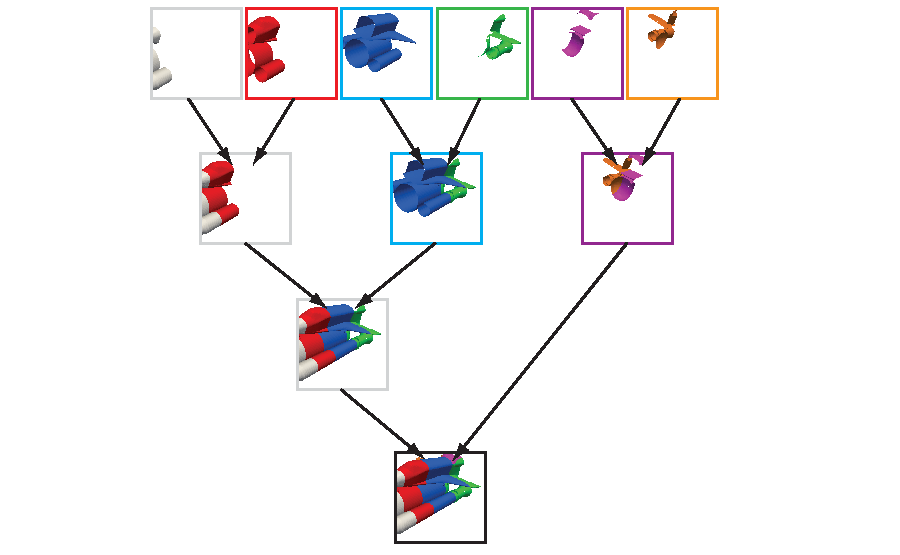
\includegraphics{images/BinaryTree}
  \caption[Tree composite network.]{Tree composite network.  Arrows
    represent the passing of data from one stage to the next.  Processes
    receiving multiple images composite them together.}
  \label{fig:BinaryTree}
\end{figure}

The tree compositing algorithm is organized in stages.  At each stage the
processes pair up.  One of the processes sends its data to its pair and
then drops out of the computation.  The receiving process combines the two
images (using the \index{compositing~operation}compositing operation
described in
Chapter~\ref{sec:Customizing_Compositing:Compositing_Operation}) and
continues to the next stage.  Processing continues until there is only one
image (and one process) remaining.

As just defined, the tree composite algorithm only handles process counts
that are a power of two (that is, the number of processes is equal to $2^i$
for some integer $i$).  \IceT handles non-powers of two gracefully.  At any
stage where the number of processes is not even and one of the processes
cannot be paired, that leftover process does nothing for that stage but
then continues to participate in the next stage.  An example of this can be
seen in the second stage of Figure~\ref{fig:BinaryTree}.

The advantages of tree composite are its regular and efficient data
transfers.  The limiting factor of tree compositing is that at each stage
of the algorithm half of the processes drop out of the computation.  Thus,
for more than a few processes tree compositing provides poor process
utilization.

\index{binary~tree~composite|)}
\index{tree~composite|)}
\index{compositing!tree|)}

\subsection{Binary-Swap Compositing}

\index{compositing!binary~swap|(}
\index{binary~swap~composite|(}

The second single image compositing algorithm provided by \IceT is the
\keyterm{binary-swap} algorithm.  The binary-swap composite sub-strategy is
selected by calling \CFunc{icetSingleImageStrategy} with
\CEnum{ICET\_SINGLE\_IMAGE\_STRATEGY\_BINARY\_SWAP}.  The basic network for
binary-swap composite is shown in Figure~\ref{fig:BinarySwap}

\begin{figure}
  \centering
  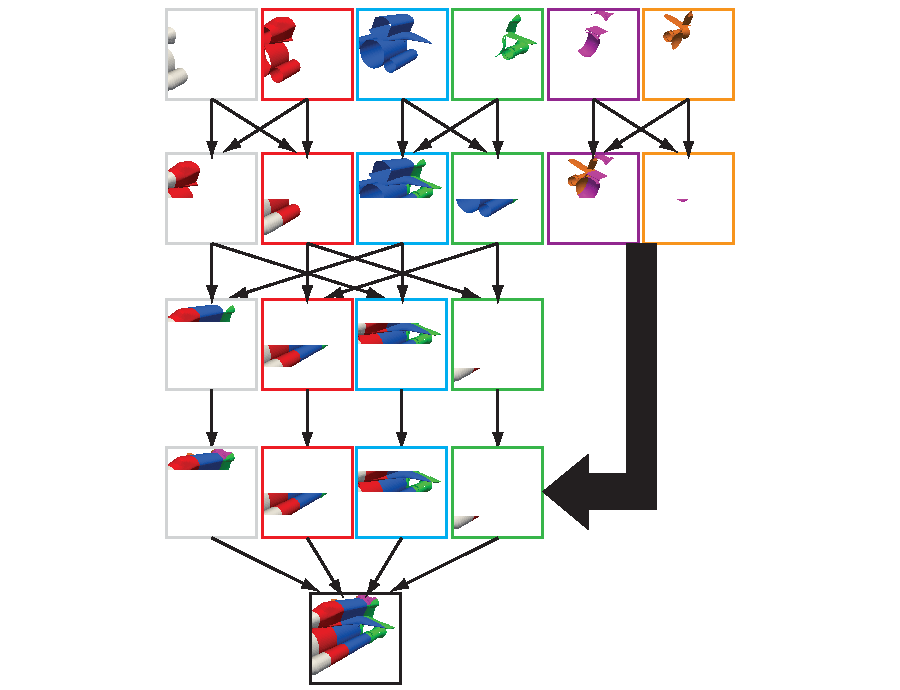
\includegraphics{images/BinarySwap}
  \caption[Binary-swap composite network.]{Binary-swap composite network.
    Arrows represent the passing of data from one stage to the next.
    Processes receiving multiple images composite or stitch them together.
    At most stages each process divides its image data and distributes it.
    The distribution of image data can be inferred from the target images.}
  \label{fig:BinarySwap}
\end{figure}

Like tree compositing, binary swap is organized in stages, and at each
stage the processes pair up.  However, rather than have one process send
all the data to the other, the image space is divided in two and the
processes swap image data so that each process has all the data for part of
the image.  At the next stage, the processes pair up again, but with
different partners that have the same partition of the image.  Processing
continues until each of the $N$ processes have an image $1/N$ the size of
the original image.  At this point, all the processes send their sub-image
to the display processes where the images are stitched together.

As just defined, the binary-swap composite algorithm only handles processes
that are a power of two (that is, the number of processes is equal to $2^i$
for some integer $i$).  Some binary-swap implementations handle non-powers
of two by reducing the problem to the next largest power of two and
dropping the leftover processes, but \IceT handles non-powers of two more
gracefully than that.  Instead, \IceT first finds the largest group of
processes that is a power of two, makes a partition out of them, then finds
the next largest group of processes that remain that is a power of two,
makes a partition out of them, and so on.  Each partition runs binary-swap
independently up to the point where each process has its own piece of data.
At this point, the smaller partitions send their image data to processes of
the larger partitions, dividing up images where necessary.  The largest
partition then finishes the compositing in the normal way by collecting all
of the pieces.

An example of compositing with a non-power of two is given in
Figure~\ref{fig:BinarySwap}.  The six processes are partitioned first into
a group of 4 and then into a group of 2.  After swapping, the processes in
the smaller group send images to the larger group.  In this case, the purple
process sends image data to the gray and blue processes, and the orange
process sends to the red and green processes.

Like tree composite, binary swap exhibits regular and efficient data
transfers.  In addition, binary swap involves the use of all the processes
throughout most of the compositing.  Consequently, binary swap exhibits
very good process utilization and scaling with respect to the number of
processes on which it is run.

The most inefficient part of binary swap is the collection of image
fragments at the end, which is an extra step that tree composite does not
need to take.  Most of the time the better parallel efficiency of binary
swap over tree composite more than compensates for the extra collection
step.

\index{binary~swap~composite|)}
\index{compositing!binary~swap|)}

\subsection{Radix-k Compositing}

\index{compositing!radix-k|(}
\index{radix-k~composite|(}

The third single image compositing algorithm provided by \IceT is the
\keyterm{radix-k} algorithm.  The radix-k composite sub-strategy is
selected by calling \CFunc{icetSingleImageStrategy} with
\CEnum{ICET\_SINGLE\_IMAGE\_STRATEGY\_RADIXK}.  An example communication
network for radix-k is shown in Figure~\ref{fig:RadixK}.

\begin{figure}
  \centering
  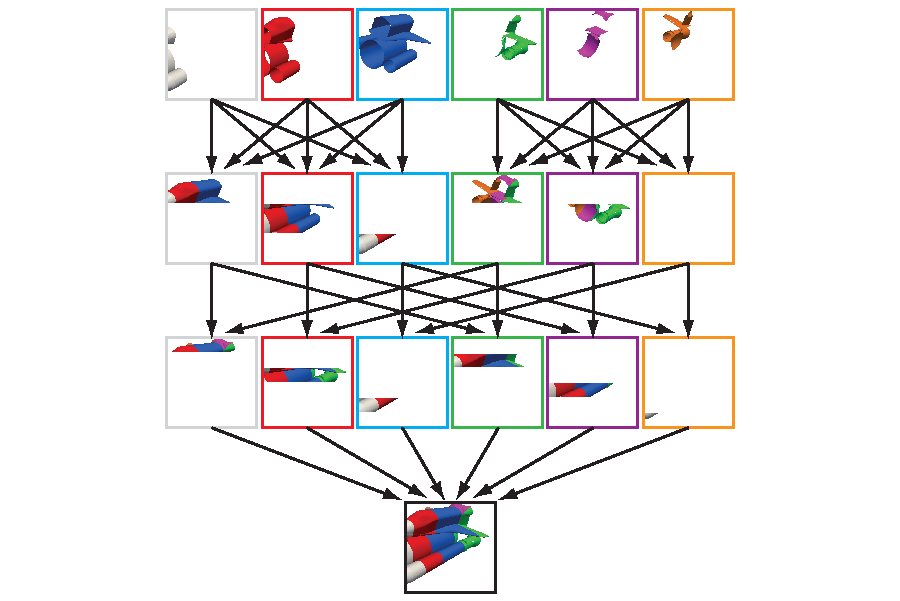
\includegraphics{images/RadixK}
  \caption[Radix-k composite network.]{Radix-k composite network using a
    round of $k=3$ and then a round of $k=2$.  Arrows represent the passing
    of data from one stage to the next.  Processes receiving multiple
    images composite or stitch them together.  The distribution of image
    data can be inferred from the target images.}
  \label{fig:RadixK}
\end{figure}

Radix-k compositing is similar to binary swap.  Both algorithms are
organized in stages.  However, where in binary swap processes pair up in
groups of 2, radix-k groups processes in arbitrary (but consistent) groups
of size $k$.  Within each group, the image is split into $k$ pieces, each
piece is assigned to a process in the group, and all image pieces are sent
to the assigned process.  At the end of the stage, all processes with the
same image piece are collected and recursed into.  The binary-swap
algorithm is a special case of radix-k with $k=2$ for every stage.

Using radix-k with $k>2$ offers two advantages.  First, some high speed
interconnects work more efficiently when there is more than one message
being transferred over the network a time.  Second, when a process is
receiving more than one image piece at a time it has the opportunity to
overlap pixel blending with the data transfer.  As soon as the first image
comes in it can be blended with the local image while the subsequent images
are still in transit.  However, the total number of messages created grows
quadratically with $k$, so too large a value will make the communication
less efficient.

The $k$ value to use for each round is automatically determined by the
number of processes participating in compositing.  The $k$ values can be
indirectly controlled by setting the \CEnum{ICET\_MAGIC\_K} environment
variable.  When set, \IceT will pick $k$ values as close as the
\CEnum{ICET\_MAGIC\_K} value as possible.  If the \CEnum{ICET\_MAGIC\_K}
value is not set, then a hard-coded target $k$ value is used, which can be
set at compile time with the \CEnum{ICET\_MAGIC\_K} \index{CMake}CMake
variable.

For more details on the radix-k algorithm, see the following paper.

\begin{quote}
  Tom Peterka, David Goodell, Robert Ross, Han-Wei Shen, and Rajeev Thakur.
  ``A Configurable Algorithm for Parallel Image-Compositing Applications,''
  In \emph{Proceedings of the Conference on High Performance Computing
    Networking, Storage and Analysis (SC '09)}, November 2009,
  DOI=10.1145/1654059.1654064.
\end{quote}

\index{radix-k~composite|)}
\index{compositing!radix-k|)}

\subsection{Automatic Algorithm Selection}

\index{automatic~composite~selection|(}
\index{compositing!automatic~selection|(}

\IceT also supports the automatic selection of the single image
sub-strategy.  This automatic selection is enabled by calling
\CFunc{icetSingleImageStrategy} with
\CEnum{ICET\_SINGLE\_IMAGE\_STRATEGY\_AUTOMATIC}. (It is also the default
for the single image strategy.)

The automatic selection attempts to guess at the best strategy.  The
intension is that \IceT can internally pick the best strategy depending on
how the compositing is being used.  For example, through some empirical
studies, we found that the binary tree algorithm was more efficient than
binary swap on less then 8 processes and less efficient on more than 8
processes.  Consequently, \IceT automatically switches between the two
algorithms based on the amount of processes involved in the compositing.

\index{compositing!automatic~selection|)}
\index{automatic~composite~selection|)}

\subsection{Ordered Compositing}

\index{compositing!ordered|(}

In some applications, the order in which images are composited together
makes a difference (see the Volume Rendering section in
Chapter~\ref{sec:Customizing_Compositing:Volume_Rendering}).  The details
on how ordered compositing is achieved is not given here, but the basic
idea for both compositing algorithms is that they first swizzle the
processes so that their order matches the order in which the images need to
be composited together.  When compositing images together, they make sure
to maintain over/under constancy based on the swizzled ranks from the
originating processes.  The networks are also managed such that no two
images are composited that are not directly ``next'' to each other (that
is, there is no image that needs to be inserted between them).

\index{compositing!ordered|)}

\index{compositing!single~image|)}
\index{single~image~composite|)}

\section{Reduce Strategy}
\label{sec:Strategies:Reduce}

\index{strategy!reduce|(}
\index{reduce~strategy|see{strategy, reduce}}
\index{reduce~to~single~tile|see{strategy, reduce}}

An effective strategy implemented in \IceT is the \keyterm{reduce to single
  tile strategy} (or simply the reduce strategy).  In this strategy, the
multi-tile composite problem is efficiently reduced to a set of single
image compositing problems, which are well studied and discussed in the
previous section.  The reduce strategy is selected by calling
\CFunc{icetStrategy} with the \CEnum{ICET\_STRATEGY\_REDUCE} argument.

\begin{figure}
  \centering
  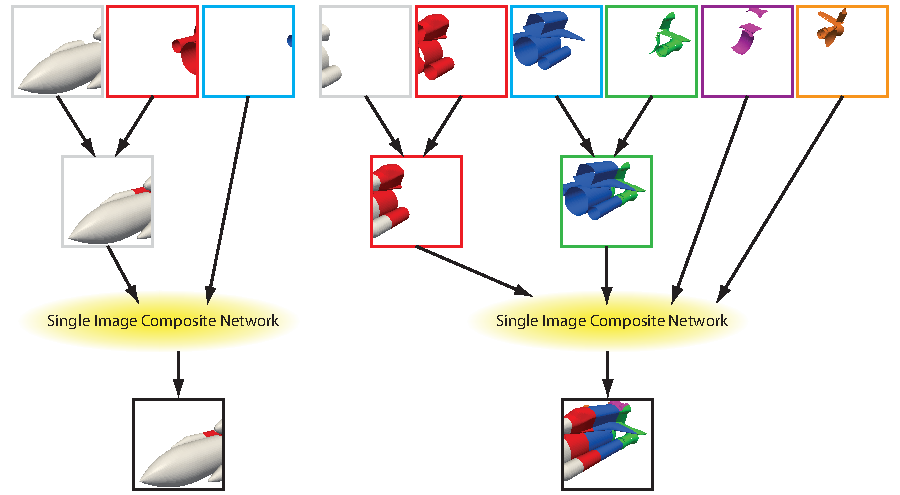
\includegraphics{images/ReduceComposite}
  \caption[Reduce strategy composite network.]{Composite network for reduce
    strategy.  Arrows represent the passing of data from one stage to the
    next.  Processes receiving multiple images composite them together.
    The single image composite network is described in a preceding
    section.}
  \label{fig:ReduceComposite}
\end{figure}

The reduce strategy is performed in two phases.  In the first phase,
processes are partitioned into groups, each of which is responsible for
compositing the image of one of the tiles.  The number of processes
assigned to each tile is proportional to the number of non-empty images
rendered for the corresponding tile.  In the example shown in
Figure~\ref{fig:ReduceComposite} there are a total of 9 non-empty images.
The left tile has 3 of the 9, that is $\frac{1}{3}$, of the images and thus
is assigned $\frac{1}{3} \times 6 = 2$ processes.  Likewise, the right
image is assigned $\frac{2}{3} \times 6 = 4$ processes.

When assigning processes to tiles, display processes and processes rendering
images to the tile are given preference.  In the example of
Figure~\ref{fig:ReduceComposite}, the gray and blue processes are assigned
to the left tile.  The remainder are assigned to the right tile.  Any image
generated by a process that does not belong to the destination tile is
transferred to a process assigned to the tile.  In the example, the three
processes that render two images, gray, red, and blue, each pass one of
their images to a process in the opposing process group.  All of these
transfers have unique senders and receivers and thus can happen
simultaneously.

In the second phase of the reduce strategy, each group of processes
independently composites its images together using one of the single image
compositing algorithms described in the preceding section.

The reduce strategy supports ordered compositing.  It does this by ensuring
in the first phase that processes receive only images that are ``near'' the
image they hold, that is, there is no other image in between the two images
in the visibility ordering.  The single image compositing algorithms of the
second phase each support their own ordered compositing.

\index{strategy!reduce|)}

\section{Split Strategy}
\label{sec:Strategies:Split}

\index{strategy!split|(}
\index{split~strategy|see{strategy, split}}
\index{tile~split~and~delegate|see{strategy, split}}

The \keyterm{tile split and delegate strategy} (or simply the split
strategy) is a simple algorithm that splits up tiles, assigns each piece to
a process, and then sends image fragments directly to the processes for
compositing.  The split strategy makes efficient use of processing
resources, but exhibits haphazard and copious message passing which can
cause issues on some high speed interconnects.  The split strategy is
selected by calling \CFunc{icetStrategy} with the
\CEnum{ICET\_STRATEGY\_SPLIT} argument.

\begin{figure}
  \centering
  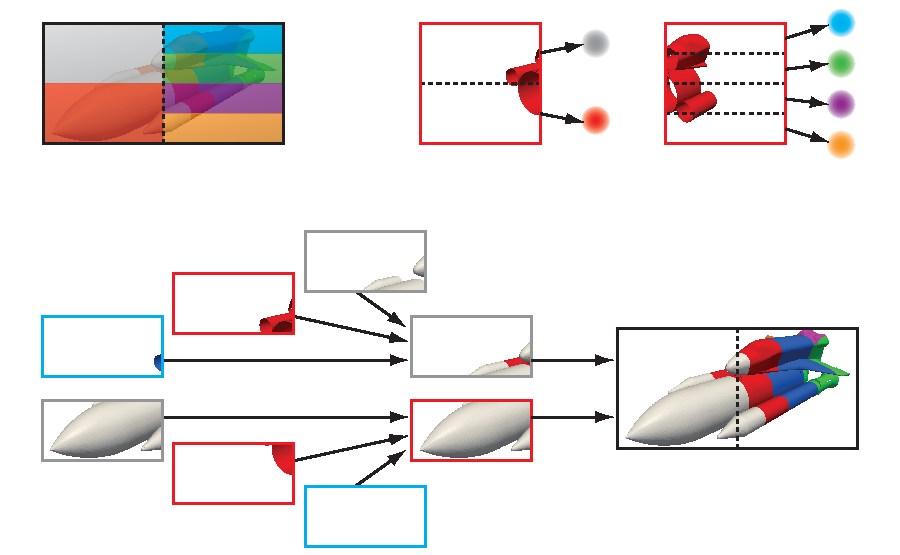
\includegraphics{images/TileSplit}
  \caption[Split strategy composite network.]{Compositing for split
    strategy.  First tiles are split and assigned to processes (upper
    left).  Then each process simultaneously sends its images to the
    responsible process (upper right) and receives all sub-images for its
    piece (bottom).  The composited pieces are then collected and stitched
    together.}
  \label{fig:TileSplit}
\end{figure}

The split strategy first assigns processes to tiles similar to how they are
assigned in the reduce strategy described previously.  That is, the number
of processes per tile is proportional to the number of non-empty images
generated for it.  Each tile is then split up evenly amongst all processes
assigned to it.  In the example in Figure~\ref{fig:TileSplit}, the upper
left image shows that the left image is split between 2 processes and the
right image is split amongst 4 processes.

On being assigned a section of tile, each process prepares to receive data
from all the sending processes using asynchronous receives.  Each process
then renders its images, splits them up, and sends the sub-images to the
corresponding process.  When a process is ready and as it receives data,
the incoming images are composited together.  Once all of the incoming
images are composited, the complete sub-image is sent to the display process
to be stitched together.

The split strategy does not support ordered compositing.  Using the split
strategy in color blending mode will fail.

\index{strategy!split|)}

\section{Virtual Trees Strategy}
\label{sec:Strategies:Vertial_Trees}

\index{strategy!virtual~trees|(}
\index{virtual~trees|see{strategy, virtual trees}}

The \keyterm{virtual trees strategy} is based on the binary tree
compositing algorithm, but performs multiple composites simultaneously to
regain some of the load balance lost in the original algorithm.  The
virtual trees strategy has nice regular communications, but still suffers
from some load imbalance, particularly when using fewer tiles and in later
stages of the algorithm.  The virtual trees strategy is selected by calling
\CFunc{icetStrategy} with the \CEnum{ICET\_STRATEGY\_VTREE} argument.

\begin{figure}
  \centering
  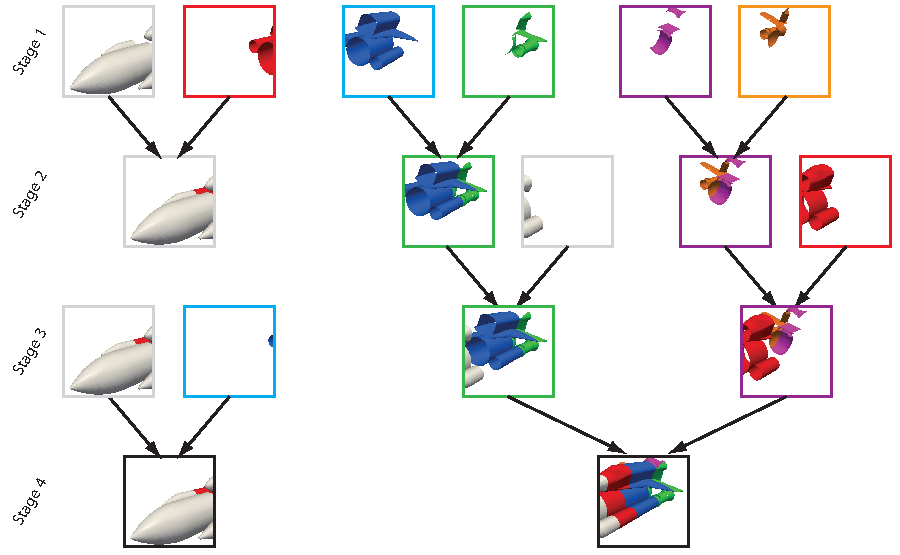
\includegraphics{images/VTrees}
  \caption[Virtual trees composite network.]{Composite network for virtual
    trees strategy.  Arrows represent the passing of data from one state to
    the next.  Processes receiving multiple images composite them
    together.}
  \label{fig:VTreesComposite}
\end{figure}

The virtual trees strategy works by creating a ``virtual'' tree for each
tile.  Contained in each tree are processes that have rendered an image for
that display tile.  The algorithm proceeds much like the binary tree
composition algorithm except that the processes float amongst the trees,
helping with the compositing as they become available.
Figure~\ref{fig:VTreesComposite} shows an example of the virtual trees
compositing.  In particular, notice that the gray process takes part in the
left tree in stage 1, then floats to take part in the right tree in stage
2, and then returns to take part in the left tree in stage 3.

When necessary, the process must keep track of multiple images belonging to
different virtual trees.  Two conserve memory, images are not rendered
until they are needed.  Also, a process can only hold two images at a time:
one that it is sending and one that it is receiving.  If a process is
holding an image for one tile, it cannot receive an image for another tile
until it sends away the image it is holding.

The virtual trees strategy does not support ordered compositing.  Using the
virtual trees strategy in color blending mode will fail.

\index{strategy!virtual~trees|)}

\section{Sequential Strategy}
\label{sec:Strategies:Sequential}

\index{strategy!sequential|(}
\index{sequential~strategy|see{strategy, sequential}}

The \keyterm{sequential strategy} sequentially addresses the tiles, but
performs parallel compositing for each tile.  The sequential strategy is
selected by calling \CFunc{icetStrategy} with the
\CEnum{ICET\_STRATEGY\_SEQUENTIAL} argument.

\begin{figure}
  \centering
  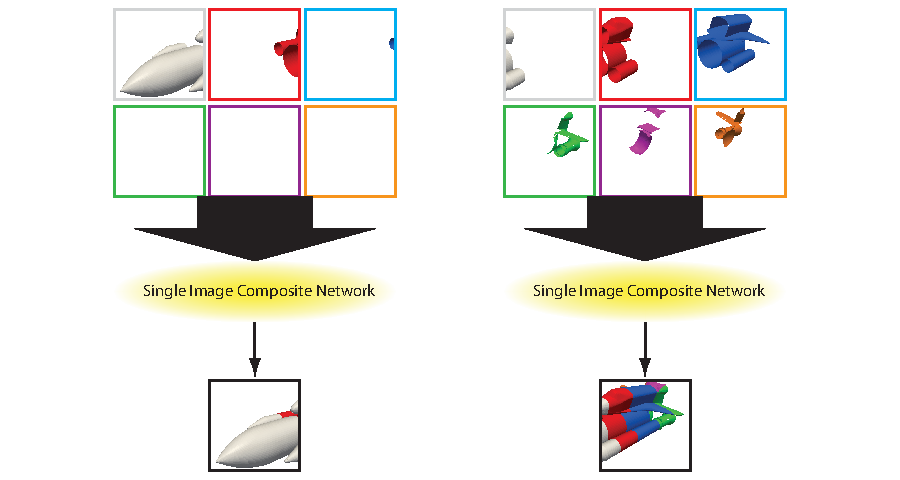
\includegraphics{images/SequentialComposite}
  \caption[Sequential compositing network.]{Composite network for
    sequential compositing.  One at a time, each tile is composited using a
    parallel single image composite network described in a previous
    section.}
  \label{fig:SequentialComposite}
\end{figure}

The sequential strategy iterates over all of the tiles.  For each tile, it
composites all the images for that tile using one of the single image
compositing algorithms described in that preceding section.  As
demonstrated in the example in Figure~\ref{fig:SequentialComposite}, images
from all processes are composited for each tile regardless of whether some
of them may be empty.

Since the single image compositing algorithms support ordered
compositing, the sequential strategy also supports ordered compositing.

The sequential strategy is most useful in the special (but common) case of
rendering to a single tile.  In this case the sequential strategy can skip
much of the global collective communication necessary for other strategies
that must manage the sparse collection of tiles.

\index{strategy!sequential|)}

\section{Direct Send Strategy}
\label{sec:Strategies:DirectSend}

\index{strategy!direct|(}
\index{direct~send~strategy|see{strategy, direct}}

The \keyterm{direct send strategy} is the simplest of all the strategies.
Each process simply renders its images and sends them directly to the
display process where the images get composited, as shown in
Figure~\ref{fig:DirectSend}.  The direct send strategy is selected by
calling \CFunc{icetStrategy} with the \CEnum{ICET\_STRATEGY\_DIRECT}
argument.

\begin{figure}
  \centering
  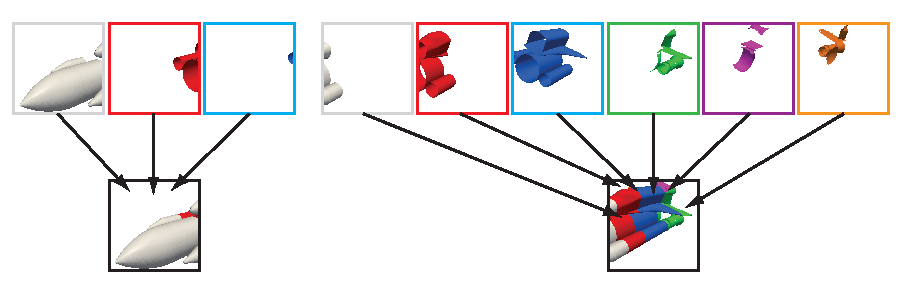
\includegraphics{images/DirectSend}
  \caption[Direct send compositing network.]{Composite network for direct
    send compositing.  Arrows represent the passing of data from one
    process to another.  Receiving process composite all incoming images
    together.}
  \label{fig:DirectSend}
\end{figure}

The direct send strategy is usually a poor performer.  It was designed as a
low watermark to compare to other compositing strategies.  The direct send
strategy does, however, support ordered compositing.

\index{strategy!direct|)}

\section{Implementing New Strategies}
\label{sec:Strategies:New}

The \IceT API was written while its strategies were being developed.  As
such, the design yields for the relatively simplistic addition of both new
multi-tile strategies and new single-image strategies.  This section will
provide the basic overview of how to add a new strategy.  It is probably
easiest to start by modifying your \IceT source to insert your own strategy
in the \textC{src/strategies} directory of the \IceT source distribution.

A strategy in \IceT is created by simply defining a function that performs
the operation.  A multi-tile strategy (one selected with
\CFunc{icetStrategy}) should take no arguments and return an
\CType{IceTImage}.  Thus, a new multi-tile strategy function would look
something like this.  (The following sections will provide details on
performing the individual tasks of the implementation.)

\begin{code}
IceTImage icetCustomMultiTileCompose(void)
{
    /* Render images. */
    /* Transfer data. */
    /* Composite pixels. */
    /* Store results in image. */
    return image;
}
\end{code}

To expose the strategy from the \IceT interface, add an identifier to
\textC{IceT.h} starting with \textC{ICET\_STRATEGY\_} to the list of
existing strategy identifiers.  Then modify the functions in
\textC{src/strategies/select.c} to expose this new identifier to the rest
of the \IceT library.  In particular, add your new identifier to the switch
statements in the following functions.

\begin{description}
\item[\CFuncExternal{icetStrategyValid}] Simply add your identifier to the
  list so that \IceT can verify that your strategy is defined.
\item[\CFuncExternal{icetStrategyNameFromEnum}] Add a short human-readable
  name for your strategy.  This is the string returned from
  \CFunc{icetGetStrategyName}.
\item[\CFuncExternal{icetStrategySupportsOrder}] Return \CEnum{ICET\_TRUE}
  if your strategy can properly composite based on the ordering given in
  \CEnum{ICET\_COMPOSITE\_ORDER}.  Return \CEnum{ICET\_FALSE} otherwise.
  This value gets stored in the \CEnum{ICET\_STRATEGY\_SUPPORTS\_ORDERING}.
\item[\CFuncExternal{icetInvokeStrategy}] Call the function that invokes
  your strategy's image compositing (\textC{icetCustomMultiTileCompose} in
  the example above).
\end{description}

The process for creating a single-image strategy (one selected with
\CFunc{icetSingleImageStrategy} is similar.  The first step is define a
function that performs the compositing.  However, the single-image
composite function takes arguments that define the image to composite and
the group of processes contributing.  A new single-image strategy function
would look something like this.

\begin{code}
void icetCustomSingleImageCompose(IceTInt *compose_group, IceTInt group_size,
                                  IceTInt image_dest,
                                  IceTImage image)
{
    /* Transfer data. */
    /* Composite pixels. */
    /* Store results in image. */
}
\end{code}

The first argument, \CArg{compose\_group}, is an array of process ranks.
The pixels are to be composited in the order specified in this array.  The
second argument, \CArg{group\_size}, specifies how many processes are
contributing to the image and also specifies the length of
\CArg{compose\_group}.  The third argument, \CArg{image\_dest}, specifies
the process in which the final composed image should be placed.  It is an
index into \CArg{compose\_group}, not the actual rank of the process.  The
final argument, \CArg{image} contains the input images to be composited
together.  It is also used to store the results of the compositing.  The
process with rank \textC{\CArg{compose\_group}[\CArg{image\_dest}]} fills
\CArg{image} with the resulting composited image.

To expose the single-image strategy from the \IceT interface, add an
identifier to \textC{IceT.h} starting with
\textC{ICET\_SINGLE\_IMAGE\_STRATEGY\_} to the list of existing
single-image strategy identifiers.  Then modify the functions in
\textC{src/strategies/select.c} to expose this new identifier to the rest
of the \IceT library.  In particular, add your new identifier to the switch
statements in the following functions.

\begin{description}
\item[\CFuncExternal{icetSingleImageStrategyValid}] Simply add your
  identifier to the list so that \IceT can verify that your strategy is
  defined.
\item[\CFuncExternal{icetSingleImageStrategyNameFromEnum}] Add a short
  human-readable name for your strategy.  This is the string returned from
  \CFunc{icetGetSingleImageStrategyName}.
\item[\CFuncExternal{icetInvokeSingleImageStrategy}] Call the function that
  invokes your strategy's image compositing
  (\textC{icetCustomSingleImageCompose} in the example above).
\end{description}

\subsection{Internal State Variables for Compositing}

The strategy compose functions are expected to get many of its parameters
and other relevant information from the \IceT state.  Many of the relevant
state variables are described in the documentation for the \CFunc{icetGet}
functions (as well as elsewhere throughout this document).  There are also
several ``hidden'' state variables for internal use.  The ones specifically
useful for within a composite function are listed here (along with the
variable type, number of entries, and a description).  Note that these
state variables generally should be read from, not written to.

\begin{Description}[xxxxxxxx]
\item[\CEnum{ICET\_ALL\_CONTAINED\_TILES\_MASKS}] (boolean,
  \CEnum{ICET\_NUM\_TILES} $\times$ \CEnum{ICET\_NUM\_PROCESSES}) Contains
  an appended list of \CEnum{ICET\_CONTAINED\_TILES\_MASK} variables for
  all processes.  Given process $p$ and tile $t$, the entry at
  $(\CEnum{ICET\_NUM\_TILES} \times p)+t$ contains the flag describing
  whether process $p$ renders a non-blank image for tile $t$.  This
  variable is the same on all processes.  This state variable is \emph{not}
  set when using the \index{strategy!sequential}sequential strategy.
\item[\CEnum{ICET\_CONTAINED\_TILES\_LIST}] (integer,
  \CEnum{ICET\_NUM\_CONTAINED\_TILES}) All the tiles into which the local
  geometry projects.  In other words, this is the list of tiles which will
  not be empty after local rendering.  The local processor should generate
  images for these tiles and participate in the composition of them.
\item[\CEnum{ICET\_CONTAINED\_TILES\_MASK}] (boolean,
  \CEnum{ICET\_NUM\_TILES}) This is a list of boolean flags, one per tile.
  The flag is true if the local geometry projects onto the tile (that is,
  the local render will not be empty for that tile) and false otherwise.
  This gives the same information as \CEnum{ICET\_CONTAINED\_TILES\_LIST},
  but in a different way that can be more convenient in some circumstances.
\item[\CEnum{ICET\_CONTAINED\_VIEWPORT}] (integer, 4) Describes the region
  of the viewport that the geometry being rendered locally projects onto.
  The bounds of the data (given by \CFunc{icetBoundingBox} or
  \CFunc{icetBoundingVertices}) projected onto the tiled display determines
  the region of the tiled display the data covers.  The values in the
  four-tuple correspond to x, y, width, and height, respectively, of the
  projection in global pixel coordinates.  This variable in conjunction
  with the \CEnum{ICET\_NEAR\_DEPTH} and \CEnum{ICET\_FAR\_DEPTH} give the
  full 3D projection of the local data in window space.
\item[\CEnum{ICET\_FAR\_DEPTH}] (double, 1) The maximum depth value of the
  local geometry after projection.  See \CEnum{ICET\_CONTAINED\_VIEWPORT}
  for more details.
\item[\CEnum{ICET\_IS\_DRAWING\_FRAME}] (boolean, 1) Set to true while in a
  call to \CFunc{icetDrawFrame} or \CFunc{icetGLDrawFrame} and set to false
  otherwise.  This should always be set to true while the compose function
  is being executed.
\item[\CEnum{ICET\_MODELVIEW\_MATRIX}] (double, 16) The current modelview
  matrix as passed to \CFunc{icetDrawFrame} or read from \OpenGL at the
  invocation of \CFunc{icetGLDrawFrame}.
\item[\CEnum{ICET\_NEAR\_DEPTH}] (double, 1) The minimum depth value of the
  local geometry after projection.  See \CEnum{ICET\_CONTAINED\_VIEWPORT}
  for more details.
\item[\CEnum{ICET\_NUM\_CONTAINED\_TILES}] (integer, 1) The number of tiles
  into which the local geometry projects.  This is the length of the
  \CEnum{ICET\_CONTAINED\_TILES\_LIST} variable.
\item[\CEnum{ICET\_PROJECTION\_MATRIX}] (double, 16) The current projection
  matrix as passed to \CFunc{icetDrawFrame} or read from \OpenGL at the
  invocation of \CFunc{icetGLDrawFrame}.
\item[\CEnum{ICET\_TILE\_CONTRIB\_COUNTS}] (integer,
  \CEnum{ICET\_NUM\_TILES}) For each tile, provides the number of processes
  that will produce a non-empty image for that tile.  This state variable
  is \emph{not} set when using the \index{strategy!sequential}sequential
  strategy.
\item[\CEnum{ICET\_TOTAL\_IMAGE\_COUNT}] (integer, 1) The total number of
  non-empty images produced by all processes for all tiles.  This variable
  is the sum of all entries in \CEnum{ICET\_TILE\_CONTRIB\_COUNTS}.  This
  state variable is \emph{not} set when using the
  \index{strategy!sequential}sequential strategy.
\end{Description}

\label{manpage:icetUnsafeStateGet}
In addition to several internal state variables, \IceT also has several
internal functions for accessing them.  The most important set for
implementing a strategy is the \CFunc{icetUnsafeStateGet} suite of
functions, which are defined in the
\index{IceTDevState.h}\textC{IceTDevState.h} header file.

\begin{Table}{4}
  \textC{IceTDouble *}&\icetUnsafeStateGetDouble\textC{(}&\textC{IceTEnum}&\CArg{pname}\quad\textC{);} \\
  \textC{IceTFloat *}&\icetUnsafeStateGetFloat\textC{(}&\textC{IceTEnum}&\CArg{pname}\quad\textC{);} \\
  \textC{IceTInt *}&\icetUnsafeStateGetInteger\textC{(}&\textC{IceTEnum}&\CArg{pname}\quad\textC{);} \\
  \textC{IceTBoolean *}&\icetUnsafeStateGetBoolean\textC{(}&\textC{IceTEnum}&\CArg{pname}\quad\textC{);} \\
  \textC{IceTVoid **}&\icetUnsafeStateGetPointer\textC{(}&\textC{IceTEnum}&\CArg{pname}\quad\textC{);}
\end{Table}

The implementation for the \CFunc{icetGet} functions is to copy the data
into a memory buffer you provide, performing type conversion as necessary.
The \CFunc{icetUnsafeStateGet} functions simply return the internal pointer
where the data is stored.  This can be faster and more convenient (since
you do not have to allocate your own memory), but is unsafe in two ways.
First, if the state variable is changed, the pointer you receive can become
invalid.  Second, no type conversion is performed.  You have to make sure
that you request a pointer of the correct type (or you will get an error).
Since the state setting functions are hidden from the end user API, it is
possible to manage these erroneous conditions.

\subsection{Memory Management}
\label{sec:Strategies:New:Memory_Management}

Compositing algorithms by their nature require buffers of memory of
non-trivial size to hold images, among other data, that are not needed in
between calls to the compositing.  One approach is to simply use the
standard C \CFuncExternal{malloc} and \CFuncExternal{free} functions.
However, some implementations of
\CFuncExternal{malloc}/\CFuncExternal{free} are not always efficient, and
even the best implementations can have a tendency to fragment memory over
time as large buffers are allocated and released.

During typical \IceT operation, a strategy (whether it be a multi-tile
strategy or a single-image strategy) is invoked multiple times.  Each
invocation will require multiple buffers to manipulate images and other
data.  One way to do this is to allocate these buffers as needed and
free them by the end of the invocation.  However, this can lead to
the inefficiencies and memory fragmentation previously mentioned.  It is
also problematic when returning an image buffer as the responsibility for
deallocating the buffer becomes undefined.

A better approach is to allocate the buffers as needed and then keep the
buffers around for the next invocation of the strategy.  This approach
requires a certain amount of overhead to check when buffers need to be
allocated or resized and when they can be freed.  \IceT uses its own state
mechanism to assist in managing memory buffers.  You do this by creating a
\index{state~buffer}\keyterm{state buffer}, a buffer attached to a state
variable.  This is done with the \CFunc{icetGetStateBuffer} function, which
is defined in \index{IceTDevState.h}\textC{IceTDevState.h}.

\label{manpage:icetGetStateBuffer}
\begin{Table}{3}
  \textC{IceTVoid *}\CFunc{icetGetStateBuffer}\textC{(}&\textC{IceTEnum}&\CArg{pname}\textC{,} \\
  &\textC{IceTSizeType}&\CArg{num\_bytes}\quad\textC{);}
\end{Table}

The \CFunc{icetGetStateBuffer} takes a state variable and a buffer size in
bytes.  It then checks to see if a buffer of the appropriate size has
already been allocated to that state variable.  If so, it is returned.  If
not, a new buffer is allocated and returned.  There are also similar
functions called \CFunc{icetGetStateBufferImage} and
\CFunc{icetGetStateBufferSparseImage}, described in the following section,
that allocate image buffers.

Because each buffer is assigned to a state variable, it is important to
assign the buffer to a state variable that is both valid and unused by
other \IceT components.  To this end, there are several state variables
reserved for multi-tile strategies or single-image strategies.  The state
variables for multi-tile strategies are named
\CEnum{ICET\_STRATEGY\_BUFFER}\textC{\_$i$} numbered from 0 to 15.  That
is, \CEnum{ICET\_STRATEGY\_BUFFER\_0}, \CEnum{ICET\_STRATEGY\_BUFFER\_1},
and so on up to \CEnum{ICET\_STRATEGY\_BUFFER\_15}.

By convention, your multi-tile strategy implementation should start by
creating \textC{\#define} enumerations that alias these variables to
logical names for the buffers.  This will help prevent confusion or
accidental sharing of buffers.  Also by convention, try to make the largest
buffers ``first'' (that is, \CEnum{ICET\_STRATEGY\_BUFFER\_0} has the
largest buffer, \CEnum{ICET\_STRATEGY\_BUFFER\_1} has the next largest, and
so on) so that if the strategy is changed, the large buffers will most
likely be shared.

As an example, consider the following code taken from the virtual trees
strategy implementation that aliases the buffer state variables it uses.

\begin{code}
#define VTREE_IMAGE_BUFFER              ICET_STRATEGY_BUFFER_0
#define VTREE_IN_SPARSE_IMAGE_BUFFER    ICET_STRATEGY_BUFFER_1
#define VTREE_OUT_SPARSE_IMAGE_BUFFER   ICET_STRATEGY_BUFFER_2
#define VTREE_INFO_BUFFER               ICET_STRATEGY_BUFFER_3
#define VTREE_ALL_CONTAINED_TMASKS_BUFFER ICET_STRATEGY_BUFFER_4
\end{code}

And here is an example of these buffers being allocated.

\begin{code}
sparseImageSize = icetSparseImageBufferSize(max_width, max_height);

image                = icetGetStateBufferImage(VTREE_IMAGE_BUFFER,
                                               max_width, max_height);
inSparseImageBuffer  = icetGetStateBuffer(VTREE_IN_SPARSE_IMAGE_BUFFER,
                                          sparseImageSize);
outSparseImage       = icetGetStateBufferSparseImage(
                                              VTREE_OUT_SPARSE_IMAGE_BUFFER,
                                              max_width, max_height);
info                 = icetGetStateBuffer(VTREE_INFO_BUFFER,
                                         sizeof(struct node_info)*num_proc);
all_contained_tmasks = icetGetStateBuffer(VTREE_ALL_CONTAINED_TMASKS_BUFFER,
                                    sizeof(IceTBoolean)*num_proc*num_tiles);
\end{code}

Once allocated, these buffers can be used and never need to be freed.
\IceT will handle the memory management.  However, do not expect any of
these buffers to contain the same data or even exist on the next invocation
of the strategy.  Each invocation of the strategy should call
\CFunc{icetGetStateBuffer}, \CFunc{icetGetStateBufferImage}, and
\CFunc{icetGetStateBufferSparseImage} to ensure that it has a valid buffer.

There is a separate set of state variables reserved for buffers used in
single-image strategies.  These are named
\CEnum{ICET\_SI\_STRATEGY\_BUFFER}\textC{\_$i$} numbered from 0 to 15.
That is, \CEnum{ICET\_SI\_STRATEGY\_BUFFER\_0},
\CEnum{ICET\_SI\_STRATEGY\_BUFFER\_1}, and so on up to
\CEnum{ICET\_SI\_STRATEGY\_BUFFER\_15}.  It is important \emph{not} to use
the multi-tile strategy buffer variables in a single-image strategy because
the multi-tile strategy will call the single-image strategy while it is
still operating and the single-image strategy can invalidate the buffers of
the multi-tile strategy.

\subsection{Image Manipulation Functions}

\IceT defines two image types: \CType{IceTImage} and
\CType{IceTSparseImage}.  Both image types can hold color data or depth
data or both.  The \CType{IceTImage} type stores pixels as raw data, simple
2D arrays holding color or pixel data in horizontal-major order.  The
\CType{IceTSparseImage} stores images using
\index{active-pixel~encoding}active-pixel encoding, the run length encoding
described in the Active-Pixel Encoding section of
Chapter~\ref{sec:Customizing_Compositing:Active_Pixel_Encoding}.

Both the \CType{IceTImage} type and the \CType{IceTSparseImage} type are
opaque to compositing algorithms.  \IceT provides functions for creating
and manipulating images.  Some of these functions are defined in
\index{IceT.h}\textC{IceT.h} and exposed to user code.  These exposed
functions are documented in the Image Objects section of
Chapter~\ref{sec:Basic_Usage:Image_Objects} starting on
page~\pageref{sec:Basic_Usage:Image_Objects}.  Other functions are
protected from the user level code and reserved for use by the compositing
algorithms and other parts of \IceT.  These functions are defined in
\index{IceTDevImage.h}\textC{IceTDevImage.h} and are documented here.  When
creating a compositing strategy, be sure to include both of these header
files.

\subsubsection{Creating Images}

\label{manpage:icetGetStateBufferImage}
\label{manpage:icetGetStateBufferSparseImage}
The easiest and safest way to create an image is to use the
\CFunc{icetGetStateBufferImage} function (or
\CFunc{icetGetStateBufferSparseImage} for sparse images).

\begin{Table}{3}
  \CType{IceTImage}\textC{ }\CFunc{icetGetStateBufferImage}\textC{(}&\textC{IceTEnum}&\CArg{pname}\textC{,} \\
  &\textC{IceTSizeType}&\CArg{width}\textC{,} \\
  &\textC{IceTSizeType}&\CArg{height}\quad\textC{);}
\end{Table}

\begin{Table}{3}
  \multicolumn{3}{l}{
    \CType{IceTSparseImage}\textC{ }\CFunc{icetGetStateBufferSparseImage}\textC{(}
  } \\
  \qquad\qquad\qquad\qquad\qquad\qquad\qquad\qquad\qquad\qquad\qquad\qquad
  &\textC{IceTEnum}&\CArg{pname}\textC{,} \\
  &\textC{IceTSizeType}&\CArg{width}\textC{,} \\
  &\textC{IceTSizeType}&\CArg{height}\quad\textC{);}
\end{Table}

Each of these functions allocates a \index{state~buffer}state buffer
(described in the previous section on Memory Management) for an image of
size \CArg{width} by \CArg{height} on the given state variable
(\CArg{pname}), and returns an initialized image object.  The image object
is allocated and initialized for the color and depth formats specified by
the \CEnum{ICET\_COLOR\_FORMAT} and \CEnum{ICET\_DEPTH\_FORMAT} state
variables.  Here is some code taken from the virtual trees strategy
implementation that demonstrates the use of these functions.

\begin{code}
image                = icetGetStateBufferImage(VTREE_IMAGE_BUFFER,
                                               max_width, max_height);
outSparseImage       = icetGetStateBufferSparseImage(
                                              VTREE_OUT_SPARSE_IMAGE_BUFFER,
                                              max_width, max_height);
\end{code}

\label{manpage:icetImageSetDimensions}
\label{manpage:icetSparseImageSetDimensions}
After an image is allocated, it is possible to resize the image, but only
to dimensions that are less than or equal to those for which the image was
created. This is done with the \CFunc{icetImageSetDimensions} or
\CFunc{icetSparseImageSetDimensions} function.

\begin{Table}{3}
  \textC{void }\CFunc{icetImageSetDimensions}\textC{(}&\CType{IceTImage}&\CArg{image}\textC{,} \\
  &\textC{IceTSizeType}&\CArg{width}\textC{,} \\
  &\textC{IceTSizeType}&\CArg{height}\quad\textC{);} \\
\end{Table}

\begin{Table}{3}
  \textC{void }\CFunc{icetSparseImageSetDimensions}\textC{(}&\CType{IceTSparseImage}&\CArg{image}\textC{,} \\
  &\textC{IceTSizeType}&\CArg{width}\textC{,} \\
  &\textC{IceTSizeType}&\CArg{height}\quad\textC{);} \\
\end{Table}

These functions do not resize the internal buffer of the image.  Rather,
they set the internal width and height parameters of the image and reuse
the original (and potentially larger than necessary) buffer.  This is why
they cannot be used to size the image larger than the original buffer
allocation.  It is for this reason that it is typical for a multi-tile
strategy to create images of size \CEnum{ICET\_TILE\_MAX\_WIDTH} and
\CEnum{ICET\_TILE\_MAX\_HEIGHT}.  A well designed compositing algorithm
should never need more space than that.  Likewise, it is typical for a
single-image strategy to create images of the same size as the input
image.

\label{manpage:icetImageBufferSize}
\label{manpage:icetSparseImageBufferSize}
It is sometimes necessary to know the size of buffer required to store
image data.  This most often occurs when allocating buffers to receive
images (as described in detail in the following section on Transferring
Images starting on
page~\pageref{sec:Strategies:New:Communications:Transferring_Images}).
Getting the necessary buffer size is done with the
\CFunc{icetImageBufferSize} and \CFunc{icetSparseImageBufferSize}
functions.

\begin{Table}{3}
  \textC{IceTSizeType }\CFunc{icetImageBufferSize}\textC{(}&\textC{IceTSizeType}&\CArg{width}\textC{,} \\
  &\textC{IceTSizeType}&\CArg{height}\quad\textC{);}
\end{Table}

\begin{Table}{3}
  \textC{IceTSizeType }\CFunc{icetSparseImageBufferSize}\textC{(}&\textC{IceTSizeType}&\CArg{width}\textC{,} \\
  &\textC{IceTSizeType}&\CArg{height}\quad\textC{);}
\end{Table}

Each of these functions returns the \emph{maximum} number of bytes required
to store the image of the given dimensions and the formats specified by the
\CEnum{ICET\_COLOR\_FORMAT} and \CEnum{ICET\_DEPTH\_FORMAT} state
variables.

\label{manpage:icetImageAssignBuffer}
\label{manpage:icetSparseImageAssignBuffer}
It is also possible, although discouraged, to convert a previously
allocated buffer into an image object with one of the following functions.

\begin{Table}{3}
  \CType{IceTImage}\textC{ }\CFunc{icetImageAssignBuffer}\textC{(}&\textC{IceTVoid *}&\CArg{buffer}\textC{,} \\
  &\textC{IceTSizeType}&\CArg{width}\textC{,} \\
  &\textC{IceTSizeType}&\CArg{height}\quad\textC{);}
\end{Table}

\begin{Table}{3}
  \multicolumn{3}{l}{
    \CType{IceTSparseImage}\textC{ }\CFunc{icetSparseImageAssignBuffer}\textC{(}
  } \\
  \qquad\qquad\qquad\qquad\qquad\qquad\qquad\qquad\qquad\qquad\qquad\qquad
  &\textC{IceTVoid *}&\CArg{buffer}\textC{,} \\
  &\textC{IceTSizeType}&\CArg{width}\textC{,} \\
  &\textC{IceTSizeType}&\CArg{height}\quad\textC{);}
\end{Table}

In each case it is assumed that the buffer is at least as large as that
indicated by the \CFunc{icetImageBufferSize} or
\CFunc{icetSparseImageBufferSize} function.

It is fairly common to need to clear an image.  This is common in a
multi-tile strategy when returning an image for which no geometry is
rendered.  \IceT provides convenience functions for setting all the data in
an image to the background color.

\label{manpage:icetClearImage}
\begin{Table}{3}
  \textC{void }\CFunc{icetClearImage}\textC{(}&\CType{IceTImage}&\CArg{image}\quad\textC{);}
\end{Table}

\label{manpage:icetClearSparseImage}
\begin{Table}{3}
  \textC{void }\CFunc{icetClearSparseImage}\textC{(}&\CType{IceTSparseImage}&\CArg{image}\quad\textC{);}
\end{Table}

\subsubsection{Querying Images}

\IceT contains several functions that allow you to query basic information
about an image object such as dimensions and data formats.  Each function
takes an information object and returns the appropriate size or identifier.
(More detail for the functions that work on \CType{IceTImage} objects is
given in the Image Objects section of
Chapter~\ref{sec:Basic_Usage:Image_Objects} starting on
page~\pageref{sec:Basic_Usage:Image_Objects}.)

\begin{Table}{5}
  \textC{IceTSizeType}&\icetImageGetWidth&\textC{(}\quad\textC{const }\CType{IceTImage}&\CArg{image}&\textC{);} \\
  \textC{IceTSizeType}&\icetImageGetHeight&\textC{(}\quad\textC{const }\CType{IceTImage}&\CArg{image}&\textC{);} \\
  \textC{IceTSizeType}&\icetImageGetNumPixels&\textC{(}\quad\textC{const }\CType{IceTImage}&\CArg{image}&\textC{);}
\end{Table}

\begin{Table}{5}
  \textC{IceTEnum}&\icetImageGetColorFormat\textC{(}&\textC{const }\CType{IceTImage}&\CArg{image}&\textC{);} \\
  \textC{IceTEnum}&\icetImageGetDepthFormat\textC{(}&\textC{const }\CType{IceTImage}&\CArg{image}&\textC{);}
\end{Table}

\label{manpage:icetSparseImageGetWidth}
\label{manpage:icetSparseImageGetHeight}
\label{manpage:icetSparseImageGetNumPixels}
\begin{Table}{4}
  \multicolumn{4}{l}{
    \textC{IceTSizeType }\CFunc{icetSparseImageGetWidth}\textC{(}
  } \\
  \qquad\qquad\qquad\qquad\qquad\qquad\qquad\qquad\qquad\qquad
  &\textC{const }\CType{IceTSparseImage}&\CArg{image}&\textC{);} \\
  \multicolumn{4}{l}{
    \textC{IceTSizeType }\CFunc{icetSparseImageGetHeight}\textC{(}
  } \\
  &\textC{const }\CType{IceTSparseImage}&\CArg{image}&\textC{);} \\
  \multicolumn{4}{l}{
    \textC{IceTSizeType }\CFunc{icetSparseImageGetNumPixels}\textC{(}
  } \\
  &\textC{const }\CType{IceTSparseImage}&\CArg{image}&\textC{);}
\end{Table}

\label{manpage:icetSparseImageGetColorFormat}
\label{manpage:icetSparseImageGetDepthFormat}
\begin{Table}{4}
  \multicolumn{4}{l}{
    \textC{IceTEnum }\CFunc{icetSparseImageGetColorFormat}\textC{(}
  } \\
  \qquad\qquad\qquad\qquad\qquad\qquad\qquad\qquad\qquad\qquad
  &\textC{const }\CType{IceTSparseImage}&\CArg{image}&\textC{);} \\
  \multicolumn{4}{l}{
    \textC{IceTEnum }\CFunc{icetSparseImageGetDepthFormat}\textC{(}
  } \\
  &\textC{const }\CType{IceTSparseImage}&\CArg{image}&\textC{);}
\end{Table}

\IceT also provides several functions for retrieving data from
\CType{IceTImage} objects.  These functions are described in the Image
Objects section of Chapter~\ref{sec:Basic_Usage:Image_Objects} starting on
page~\pageref{sec:Basic_Usage:Image_Objects}.  There is no mechanism for
directly accessing the data in an \CType{IceTSparseImage}.  Instead, data
is indirectly manipulated via compression and compositing functions, which
are described in the subsequent sections.

\subsubsection{Setting Pixel Data}

There are several mechanisms for setting, changing, or copying pixel data
in \CType{IceTImage} objects.  Foremost are the \icetImageGetColor and
\icetImageGetDepth functions that return the data buffer containing the
color or depth values.

\begin{Table}{4}
  \textC{IceTUByte *}&\icetImageGetColorub&\textC{(}\quad\CType{IceTImage}&\CArg{image}\quad\textC{)}; \\
  \textC{IceTUInt *}&\icetImageGetColorui&\textC{(}\quad\CType{IceTImage}&\CArg{image}\quad\textC{)}; \\
  \textC{IceTFloat *}&\icetImageGetColorf&\textC{(}\quad\CType{IceTImage}&\CArg{image}\quad\textC{)}; \\
  \\
  \textC{IceTFloat *}&\icetImageGetDepthf&\textC{(}\quad\CType{IceTImage}&\CArg{image}\quad\textC{)};
\end{Table}

The pointers returned from these functions are shared with the
\CType{IceTImage} object itself, so writing data into the buffer will
change the image object as well.

\IceT is also able to copy data from one \CType{IceTImage} to another.  The
first function is \CFunc{icetImageCopyPixels}, which copies a contiguous
section of pixels.

\label{manpage:icetImageCopyPixels}
\begin{Table}{3}
  \textC{void }\CFunc{icetImageCopyPixels}\textC{(}&\textC{const }\CType{IceTImage}&\CArg{in\_image}\textC{,} \\
  &\textC{IceTSizeType}&\CArg{in\_offset}\textC{,} \\
  &\CType{IceTImage}&\CArg{out\_image}\textC{,} \\
  &\textC{IceTSizeType}&\CArg{out\_offset}\textC{,} \\
  &\textC{IceTSizeType}&\CArg{num\_pixels}\quad\textC{);}
\end{Table}

\CFunc{icetImageCopyPixels} copies pixel data from \CArg{in\_image} to
\CArg{out\_image}.  \CArg{in\_image} and \CArg{out\_image} must have the
same format.  Both color and depth values are copied when available.  The
data is taken from the input starting at index \CArg{in\_offset} and are
placed in the output starting at index \CArg{out\_offset}.
\CArg{num\_pixels} are copied in all.  The following example code copies
the entire contents from \textC{in\_image} to \textC{out\_image} (assuming
they have the same sizes and formats).

\begin{code}
icetImageCopyPixels(in_image, 0, out_image, 0, icetImageGetNumPixels(in_image));
\end{code}

This example copies the third row of data from the input image to the fifth
row of data in the output image.

\begin{code}
width = icetImageGetWidth(in_image);
icetImageCopyPixels(in_image, 3*width, out_image, 5*width, width);
\end{code}

This example copies the second half of pixels in \textC{in\_image} and
places it in the first part of \textC{out\_image}.  Notice that coping a
contiguous region of pixels makes it easy to divide images in halves (or
thirds, or whatevers), which is a common operation in image compositing,
without having to worry about image dimensions.

\begin{code}
num_pixels = icetImageGetNumPixels(in_image);
icetImageCopyPixels(in_image, num_pixels/2, out_image, 0, num_pixels/2);
\end{code}

A second convenience function for copying data amongst arrays is
\CFunc{icetImageCopyRegion}.  This function works much like
\CFunc{icetImageCopyPixels}, except that you specify a rectangular 2D
viewport window to copy rather than a 1D array region of pixels.

\label{manpage:icetImageCopyRegion}
\begin{Table}{3}
  \textC{void }\CFunc{icetImageCopyRegion}\textC{(}&\textC{const }\CType{IceTImage}&\CArg{in\_image}\textC{,} \\
  &\textC{const IceTInt *}&\CArg{in\_viewport}\textC{,} \\
  &\CType{IceTImage}&\CArg{out\_image}\textC{,} \\
  &\textC{const IceTInt *}&\CArg{out\_viewport}\quad\textC{);}
\end{Table}

\CArg{in\_viewport} is an array containing 4 values that specify the
rectangular region from which to copy.  The first 2 values specify the $x$
and $y$ position of the lower left corner of the region.  The second 2
values specify the width and height of the region.  \CArg{out\_viewport} is
a similar array that specifies the destination region.  The width and
height of \CArg{in\_viewport} and \CArg{out\_viewport} must be the same.
Here is a simple example of copying all the pixels from \textC{in\_image}
to \textC{out\_image}.

\begin{code}
IceTInt full_viewport[4];

full_viewport[0] = 0;
full_viewport[1] = 0;
full_viewport[2] = icetImageGetWidth(in_image);
full_viewport[3] = icetImageGetHeight(out_image);

icetImageCopyRegion(in_image, full_viewport, out_image, full_viewport);
\end{code}

This example copies a $50 \times 50$ region of pixels from the lower left
corner of \textC{in\_image} to the upper right corner of
\textC{out\_image}.

\begin{code}
IceTInt in_viewport[4], out_viewport[3];

in_viewport[0] = 0;   in_viewport[1] = 0;
in_viewport[2] = 50;  in_viewport[3] = 50;

out_viewport[0] = icetImageGetWidth(in_image) - 50;
out_viewport[1] = icetImageGetHeight(in_image) - 50;
out_viewport[2] = 50;
out_viewport[3] = 50;

icetImageCopyRegion(in_image, in_viewport, out_image, out_viewport);
\end{code}

As mentioned previously, there is a \CFunc{icetClearImage} function to
clear the contents of an image to background.  There is also another
function called \CFunc{icetImageClearAroundRegion} that sets the image to
background everywhere but in a specified 2D viewport window.

\label{manpage:icetImageClearAroundRegion}
\begin{Table}{3}
  \textC{void }\CFunc{icetImageClearAroundRegion}\textC{(}&\CType{IceTImage}&\CArg{image}\textC{,} \\
  &\textC{const IceTInt *}&\CArg{region}\quad\textC{);}
\end{Table}

Expanding on the previous example, here is code that copies a region of
pixels and then clears everything outside of this region in the
destination.

\begin{code}
icetImageCopyRegion(in_image, in_viewport, out_image, out_viewport);
icetImageClearAroundRegion(out_image, out_viewport);
\end{code}

There are no equivalent mechanisms for changing pixel data in
\CType{IceTSparseImage} objects.  Instead, data is indirectly manipulated
via compression and compositing functions, which are described in the
subsequent sections.

\subsubsection{Compressing Images}

\label{manpage:icetCompressImage}
\CFunc{icetCompressImage} converts a full \CType{IceTImage} into to more
compact \CType{IceTSparseImage}.

\begin{Table}{3}
  \textC{void }\CFunc{icetCompressImage}\textC{(}&\textC{const }\CType{IceTImage}&\CArg{image},\\
  &\CType{IceTSparseImage}&\CArg{compressed\_image}\textC{);}
\end{Table}

\label{manpage:icetCompressSubImage}
Sometimes it is convenient to break up an image into pieces, and compress
each piece.  This is common when dividing up an image to be divvied amongst
some amount of processes.  This can be most easily achieved by using the
\CFunc{icetCompressSubImage}.

\begin{Table}{3}
  \textC{void }\CFunc{icetCompressSubImage}\textC{(}&\textC{const }\CType{IceTImage}&\CArg{image},\\
  &\textC{IceTSizeType}&\CArg{offset},\\
  &\textC{IceTSizeType}&\CArg{pixels},\\
  &\CType{IceTSparseImage}&\CArg{compressed\_image}\textC{ );}
\end{Table}

\CFunc{icetCompressSubImage} compresses a region of contiguous pixels.  The
block of pixels starts \CArg{offset} pixels past the beginning of the image
and is \CArg{pixels} long.  \CArg{icetCompressImage} is almost equivalent
to calling \CArg{icetCompressSubImage} with \CArg{offset} set to $0$ and
\CArg{pixels} set to the result of \icetImageGetNumPixels.  When
compressing an image with \CFunc{icetCompressSubImage}, the output
\CType{IceTSparseImage} has its width set to the \CArg{pixels} argument and
its height set to 1.

\label{manpage:icetDecompressImage}
A sparse image can be returned to its uncompressed form with
\CFunc{icetDecompressImage}.

\begin{Table}{3}
  \multicolumn{3}{l}{\textC{void }\CFunc{icetDecompressImage}\textC{(}}\\
  \makebox[2in]{}
  &\textC{const }\CType{IceTSparseImage}&\CArg{compressed\_image}\textC{,}\\
  &\CType{IceTImage}&\CArg{image}\quad\textC{);}
\end{Table}

\subsubsection{Rendering Images}

\label{manpage:icetGetTileImage}
\label{manpage:icetGetCompressedTileImage}
A multi-tile compositing strategy is responsible for rendering images on
demand as well as compositing.  To render and retrieve the image for a
particular tile in the display, use either \CFunc{icetGetTileImage} or
\CFunc{icetGetCompressedTileImage}.

\begin{Table}{3}
  \textC{void }\CFunc{icetGetTileImage}\textC{(}&\textC{IceTInt}&\CArg{tile},\\
    &\CType{IceTImage}&\CArg{image}\quad\textC{);}
\end{Table}
\begin{Table}{3}
  \textC{void }\CFunc{icetGetCompressedTileImage}\textC{(}&\textC{IceTInt}&\CArg{tile},\\
    &\CType{IceTSparseImage}&\CArg{image}\quad\textC{);}
\end{Table}

Both functions will invoke a rendering for that tile (performing the
appropriate projection transformations) as necessary, read back the frame
buffers and store the results in an image buffer you specify.  The
difference, of course, is that \CFunc{icetGetTileImage} fills the buffer
with raw data whereas \CFunc{icetGetCompressedTileImage} will compress the
image data with \index{active-pixel~encoding}active-pixel encoding.

Although it is roughly equivalent to calling \CFunc{icetGetTileImage} and
then \CFunc{icetCompressImage}, \CFunc{icetGetCompressedTileImage} can be
much more efficient.

\subsubsection{Image Compositing}

The \IceT library contains multiple functions to locally composite two images
together.  These functions handle the complexities of dealing with
different image formats and compositing operations.

\label{manpage:icetComposite}
\begin{Table}{3}
  \textC{void }\CFunc{icetComposite}\textC{(}&\CType{IceTImage}&\CArg{destBuffer}\textC{,}\\
  &\textC{const }\CType{IceTImage}&\CArg{srcBuffer}\textC{,}\\
  &\textC{int}&\CArg{srcOnTop}\quad\textC{);}
\end{Table}

\CFunc{icetComposite} takes the images stored in \CArg{destBuffer} and
\CArg{srcBuffer}, composites them together, and stores the result in
\CArg{destBuffer}.  The compositing operation is determined by the
\CEnum{ICET\_COMPOSITE\_MODE} state variable. (See the discussion on
Compositing Operations in
Chapter~\ref{sec:Customizing_Compositing:Compositing_Operation} for
information on how the compositing operation is determined.)  If the
compositing operation is order dependent, then the Boolean argument
\CArg{srcOnTop} determines whether \CArg{srcBuffer} or \CArg{destBuffer} is
on top.

If one of your images is compressed (stored in an \CType{IceTSparseImage},
it is faster to perform the compositing operation on the compressed image
rather than decompressing first.  In fact, it is faster to composite a
compressed image than two full images because the
\index{active-pixel~encoding}active-pixel encoding allows the composite
algorithm to skip over groups of background pixels.  This gives you the
double win of faster image transfer and faster compositing.

\label{manpage:icetCompressedComposite}
\begin{Table}{3}
  \multicolumn{3}{l}{\textC{void }\CFunc{icetCompressedComposite}\textC{(}}\\
  \makebox[2.5in]{}&\CType{IceTImage}&\CArg{destBuffer}\textC{,}\\
  &\textC{const }\CType{IceTSparseImage}&\CArg{srcBuffer}\textC{,}\\
  &\textC{int}&\CArg{srcOnTop}\quad\textC{);}
\end{Table}

\CFunc{icetCompressedComposite} behaves just like \CFunc{icetComposite}
except that \CArg{srcBuffer} is a compressed image rather than a full
image.  The images in \CArg{destBuffer} and \CArg{srcBuffer} are composited
together, and the results are stored in \CArg{destBuffer}.

Many parallel compositing algorithms break images into pieces, distribute
amongst processes, and composite the pieces.  To facilitate the compositing
image pieces, \IceT provides \CFunc{icetCompressedSubComposite}.

\label{manpage:icetCompressedSubComposite}
\begin{Table}{3}
  \multicolumn{3}{l}{\textC{void }\CFunc{icetCompressedSubComposite}\textC{(}}\\
  \makebox[2.5in]{}&\CType{IceTImage}&\CArg{destBuffer}\textC{,}\\
  &\textC{IceTSizeType}&\CArg{offset}\textC{,}\\
  &\textC{const }\CType{IceTSparseImage}&\CArg{srcBuffer}\textC{,}\\
  &\textC{int}&\CArg{srcOnTop}\textC{);}
\end{Table}

The \CArg{destBuffer}, \CArg{srcBuffer} and \CArg{srcOnTop} arguments are
the same as those in \CFunc{icetCompressedComposite}.  The \CArg{offset}
argument and the number of pixels in \CArg{srcBuffer} specify a region of
contiguous pixels in \CArg{destBuffer} to perform the compositing in.

\subsection{Communications}

\IceT provides an abstract communication layer, which is described in
detail in Chapter~\ref{chap:Communicators}.  A handle to a communicator is
stored in the current context.  To make using the communicator easier, a
set of convenience functions described next is available in the
\index{IceTDevCommunication.h}\textC{IceTDevCommunication.h} include file.
All of these functions are based off of those found in the \MPI standard.
For documentation, see that for the corresponding \MPI function.  Data
types, however, are specified as one of the following \IceT data types:
\CEnum{ICET\_BOOLEAN}, \CEnum{ICET\_BYTE}, \CEnum{ICET\_SHORT},
\CEnum{ICET\_INT}, \CEnum{ICET\_SIZE\_TYPE}, \CEnum{ICET\_FLOAT}, or
\CEnum{ICET\_DOUBLE}.  There is also an \CEnum{ICET\_IN\_PLACE\_COLLECT}
identifier that takes the place of \CEnum{MPI\_IN\_PLACE} for the gather
functions (\CFunc{icetCommGather}, \CFunc{icetCommGatherv}, and
\CFunc{icetCommAllgather}).

Note that each function is missing an argument specifying the communicator.
These functions just grab the current context's communicator.  Also unlike
\MPI, these functions do not return error codes.  It is assumed that errors
are fatal.  Some functions, like \CFunc{icetCommSize},
\CFunc{icetCommRank}, and \CFunc{icetCommWaitany} use the function return
value instead of passing a value back in a pointer argument.

\label{manpage:icetCommDuplicate}
\begin{Table}{3}
  \textC{struct }\CType{IceTCommunicatorStruct}\textC{ *}\CFunc{icetCommDuplicate}\textC{(void);}
\end{Table}

\label{manpage:icetCommBarrier}
\begin{Table}{3}
  \textC{void }\CFunc{icetCommBarrier}\textC{(void);}
\end{Table}

\label{manpage:icetCommSend}
\begin{Table}{3}
  \textC{void }\CFunc{icetCommSend}\textC{(}&\textC{const void *}&\CArg{buf}\textC{,}\\
  &\textC{int}&\CArg{count},\\
  &\textC{IceTEnum}&\CArg{datatype},\\
  &\textC{int}&\CArg{dest},\\
  &\textC{int}&\CArg{tag}\quad\textC{);}
\end{Table}

\label{manpage:icetCommRecv}
\begin{Table}{3}
  \textC{void }\CFunc{icetCommRecv}\textC{(}&\textC{void *}&\CArg{buf}\textC{,}\\
  &\textC{int}&\CArg{count},\\
  &\textC{IceTEnum}&\CArg{datatype},\\
  &\textC{int}&\CArg{src},\\
  &\textC{int}&\CArg{tag}\quad\textC{);}
\end{Table}

\label{manpage:icetCommSendrecv}
\begin{Table}{3}
  \textC{void }\CFunc{icetCommSendrecv}\textC{(}&\textC{const void *}&\CArg{sendbuf}\textC{,}\\
  &\textC{int}&\CArg{sendcount}\textC{,}\\
  &\textC{IceTEnum}&\CArg{sendtype}\textC{,}\\
  &\textC{int}&\CArg{dest}\textC{,}\\
  &\textC{int}&\CArg{sendtag}\textC{,}\\
  &\textC{void *}&\CArg{recvbuf}\textC{,}\\
  &\textC{int}&\CArg{recvcount}\textC{,}\\
  &\textC{IceTEnum}&\CArg{recvtype}\textC{,}\\
  &\textC{int}&\CArg{src}\textC{,}\\
  &\textC{int}&\CArg{recvtag}\quad\textC{);}
\end{Table}

\label{manpage:icetCommGather}
\begin{Table}{3}
  \textC{void }\CFunc{icetCommGather}\textC{(}&\textC{const void *}&\CArg{sendbuf}\textC{,}\\
  &\textC{int}&\CArg{sendcount}\textC{,}\\
  &\textC{IceTEnum}&\CArg{datatype}\textC{,}\\
  &\textC{void *}&\CArg{recvbuf}\textC{,}\\
  &\textC{int}&\CArg{root}\quad\textC{);}
\end{Table}

\label{manpage:icetCommGatherv}
\begin{Table}{3}
  \textC{void }\CFunc{icetCommGatherv}\textC{(}&\textC{const void *}&\CArg{sendbuf}\textC{,}\\
  &\textC{int}&\CArg{sendcount}\textC{,}\\
  &\textC{IceTEnum}&\CArg{datatype}\textC{,}\\
  &\textC{void *}&\CArg{recvbuf}\textC{,}\\
  &\textC{const IceTSizeType *}&\CArg{recvcounts}\textC{,}\\
  &\textC{const IceTSizeType *}&\CArg{recvoffsets}\textC{,}\\
  &\textC{int}&\CArg{root}\quad\textC{);}
\end{Table}

\label{manpage:icetCommAllgather}
\begin{Table}{3}
  \textC{void }\CFunc{icetCommAllgather}\textC{(}&\textC{const void *}&\CArg{sendbuf}\textC{,}\\
  &\textC{int}&\CArg{sendcount}\textC{,}\\
  &\textC{IceTEnum}&\CArg{type}\textC{,}\\
  &\textC{void *}&\CArg{recvbuf}\quad\textC{);}
\end{Table}

\label{manpage:icetCommAlltoall}
\begin{Table}{3}
  \textC{void }\CFunc{icetCommAlltoall}\textC{(}&\textC{const void *}&\CArg{sendbuf}\textC{,}\\
  &\textC{int}&\CArg{sendcount}\textC{,}\\
  &\textC{IceTEnum}&\CArg{type}\textC{,}\\
  &\textC{void *}&\CArg{recvbuf}\quad\textC{);}
\end{Table}

\label{manpage:icetCommIsend}
\begin{Table}{3}
  \CType{IceTCommRequest}\textC{ }\CFunc{icetCommIsend}\textC{(}&\textC{const void *}&\CArg{buf}\textC{,}\\
  &\textC{int}&\CArg{count},\\
  &\textC{IceTEnum}&\CArg{datatype},\\
  &\textC{int}&\CArg{dest},\\
  &\textC{int}&\CArg{tag}\quad\textC{);}
\end{Table}

\label{manpage:icetCommIrecv}
\begin{Table}{3}
  \CType{IceTCommRequest}\textC{ }\CFunc{icetCommIrecv}\textC{(}&\textC{void *}&\CArg{buf}\textC{,}\\
  &\textC{int}&\CArg{count},\\
  &\textC{IceTEnum}&\CArg{datatype},\\
  &\textC{int}&\CArg{src},\\
  &\textC{int}&\CArg{tag}\quad\textC{);}
\end{Table}

\label{manpage:icetCommWait}
\begin{Table}{3}
  \textC{void }\CFunc{icetCommWait}\textC{(}&\CType{IceTCommRequest}\textC{ *}&\CArg{request}\quad\textC{);}
\end{Table}

\label{manpage:icetCommWaitany}
\begin{Table}{3}
  \multicolumn{3}{l}{\textC{void }\CFunc{icetCommWaitany}\textC{(}}\\
  \makebox[1.8in]{}&\textC{int}&\CArg{count},\\
  &\CType{IceTCommRequest}\textC{ *}&\CArg{array\_of\_requests}\quad\textC{);}
\end{Table}

\label{manpage:icetCommSize}
\begin{Table}{3}
  \textC{int }\CFunc{icetCommSize}\textC{(void);}
\end{Table}

\label{manpage:icetCommRank}
\begin{Table}{3}
  \textC{int }\CFunc{icetCommRank}\textC{(void);}
\end{Table}

In addition to these \MPI-like functions, \textC{IceTDevCommunication.h}
provides a couple of helper functions for finding ranks in process groups.
A group in \IceT is simply represented by an integer array that maps (via
the index) the rank in the group to the rank of the same process in the
current context's communicator.  An example of such a group is passed to
the single image strategy compose function as demonstrated in
Section~\ref{sec:Strategies:New}.

\label{manpage:icetFindRankInGroup}
\begin{Table}{3}
  \textC{int }\CFunc{icetFindRankInGroup}\textC{(}&\textC{const int *}&\CArg{group}\textC{,}\\
  &\textC{IceTSizeType}&\CArg{group\_size}\textC{,}\\
  &\textC{int}&\CArg{rank\_to\_find}\quad\textC{);}
\end{Table}

\label{manpage:icetFindMyRankInGroup}
\begin{Table}{3}
  \textC{int }\CFunc{icetFindMyRankInGroup}\textC{(}&\textC{const int *}&\CArg{group}\textC{,}\\
  &\textC{IceTSizeType}&\CArg{group\_size}\quad\textC{);}
\end{Table}

These functions provide the reverse mapping of a rank from the context's
communicator to a rank in the group.  The first form,
\CFunc{icetFindRankInGroup}, takes a \CArg{group} (and its
\CArg{group\_size}) and a \CArg{rank} and returns the index in \CArg{group}
that contains \CArg{rank}.  If \CArg{rank} is not in \CArg{group}, -1 is
returned.  \CFunc{icetFindMyRankInGroup} is similar except that it returns
the index for the local rank.  Calling \CFunc{icetFindMyRankInGroup} is
equivalent to calling \CFunc{icetFindRankInGroup} with \CArg{rank} set to
the value in the state variable \CEnum{ICET\_RANK}.

\subsubsection{Transferring Images}
\label{sec:Strategies:New:Communications:Transferring_Images}

Although the \CType{IceTImage} and \CType{IceTSparseImage} types are
opaque, \IceT provides a mechanism to transfer the data.  A pair of
functions allow you to package the data into a buffer (provided for you)
and then unpackage a buffer back into an image object.  The first of these
functions is \CFunc{icetImagePackageForSend} for \CType{IceTImage} or
\CFunc{icetSparseImagePackageForSend} for \CType{IceTSparseImage}.

\label{manpage:icetImagePackageForSend}
\begin{Table}{3}
  \textC{void }\CFunc{icetImagePackageForSend}\textC{(}&\CType{IceTImage}&\CArg{image}\textC{,} \\
  &\textC{IceTVoid **}&\CArg{buffer}\textC{,} \\
  &\textC{IceTSizeType *}&\CArg{size}\quad\textC{);}
\end{Table}

\label{manpage:icetSparseImagePackageForSend}
\begin{Table}{3}
  \textC{void }\CFunc{icetSparseImagePackageForSend}\textC{(}&\CType{IceTSparseImage}&\CArg{image}\textC{,} \\
  &\textC{IceTVoid **}&\CArg{buffer}\textC{,} \\
  &\textC{IceTSizeType *}&\CArg{size}\quad\textC{);}
\end{Table}

Both of these functions behave identically.  They return a pointer in
\CArg{buffer} to a block of raw data that can be sent opaquely via the
communications functions.  The length of this buffer in bytes is returned
in \CArg{size}.  When sending this data, send it as \CEnum{ICET\_BYTE} type
data of \CArg{size} length.  In the following example, an \textC{image} is
compressed and then its data is sent to another process.

\index{icetGetStateBufferSparseImage}
\index{icetSparseImagePackageForSend}
\index{icetCommSend}
\begin{code}
IceTSparseImage src_sparse_image;
IceTVoid *package_buffer;
IceTSizeType package_size;

src_sparse_image = icetGetStateBufferSparseImage(MYCOMPOSITE_SRC_SPARSE_IMAGE,
                                                 max_width, max_height);
icetSparseImagePackageForSend(src_sparse_image, &package_buffer, &package_size);
icetCommSend(package_buffer, package_size, ICET_BYTE, dest_rank,
             MYCOMPOSITE_FOO_TAG);
\end{code}

The companion to each package function is the unpackage function.  These
are \CFunc{icetImageUnpackageFromReceive} for \CType{IceTImage} and
\CFunc{icetSparseImageUnpackageFromReceive} for \CType{IceTSparseImage}.

\label{manpage:icetImageUnpackageFromReceive}
\begin{Table}{3}
  \CType{IceTImage}\textC{ }\CFunc{icetImageUnpackageFromReceive}\textC{(}&\textC{IceTVoid *}&\CArg{buffer}\quad\textC{);}
\end{Table}

\label{manpage:icetSparseImageUnpackageFromReceive}
\begin{Table}{3}
  \multicolumn{3}{l}{
    \CType{IceTSparseImage}\textC{ }\CFunc{icetSparseImageUnpackageFromReceive}\textC{(}
  } \\
  \makebox[4in]{}
  &\textC{IceTVoid *}&\CArg{buffer}\quad\textC{);}
\end{Table}

These functions take a buffer containing the same data provided by a
package command, create an image object, and return that object.  Note that
the buffer provided becomes part of the image.  If that buffer is destroyed
the image reverts to an undefined state.

This leads to a minor complication when receiving images.  The receiver
must allocate a raw buffer of the appropriate size and then leave it
available while the image is still in use.  This is best done by creating a
\index{state~buffer}state buffer (described in the Memory Management
section starting on page~\pageref{sec:Strategies:New:Memory_Management}).
The size necessary for these buffers is determined with the buffer size
functions, repeated here for reference.

\begin{Table}{3}
  \textC{IceTSizeType }\CFunc{icetImageBufferSize}\textC{(}&\textC{IceTSizeType}&\CArg{width}\textC{,} \\
  &\textC{IceTSizeType}&\CArg{height}\quad\textC{);}
\end{Table}

\begin{Table}{3}
  \textC{IceTSizeType }\CFunc{icetSparseImageBufferSize}\textC{(}&\textC{IceTSizeType}&\CArg{width}\textC{,} \\
  &\textC{IceTSizeType}&\CArg{height}\quad\textC{);}
\end{Table}

As a companion to the previous example, here a sparse image is received
from another process and then composited into a locally held
\textC{image}.

\index{icetSparseImageBufferSize}
\index{icetGetStateBuffer}
\index{icetCommRecv}
\index{icetSparseImageUnpackageFromReceive}
\index{icetCompressedComposite}
\begin{code}
IceTSparseImage dest_sparse_image;
IceTVoid *package_buffer;
IceTSizeType max_package_size;

max_package_size = icetSparseImageBufferSize(max_width, max_height);
package_buffer = icetGetStateBuffer(MYCOMPOSITE_DEST_SPARSE_IMAGE,
                                    max_package_size);
icetCommRecv(package_buffer, max_package_size, ICET_BYTE, src_rank,
             MYCOMPOSITE_FOO_TAG);
dest_sparse_image = icetSparseImageUnpackageFromReceive(package_buffer);
icetCompressedComposite(image, dest_sparse_image, ICET_FALSE);
\end{code}

\subsubsection{Helper Communication Functions}

\index{common.h}\textC{common.h} (found in the strategies directory)
contains some helper functions that implement common communication
patterns.  They may be helpful in implementing your strategy.

\label{manpage:icetRenderTransferFullImages}
\begin{Table}{3}
  \multicolumn{3}{l}{\textC{void }\CFunc{icetRenderTransferFullImages}\textC{(}}\\
  \makebox[2in]{}
  &\CType{IceTImage}&\CArg{image}\textC{,}\\
  &\textC{IceTVoid *}&\CArg{inSparseImageBuffer}\textC{,}\\
  &\CType{IceTSparseImage}&\CArg{outSparseImage}\textC{,}\\
  &\textC{IceTInt *}&\CArg{tile\_image\_dest}\quad\textC{);}
\end{Table}

\CFunc{icetRenderTransferFullImages} renders all the tiles that are
specified in the \CEnum{ICET\_CONTAINED\_TILES\_LIST} state array and sends
them to the processors with ranks specified in \CArg{tile\_image\_dest}.
This function is guaranteed not to deadlock so long as all processes call
it.  The function uses only memory given with the buffer arguments, and
will make its best efforts to get the graphics and network hardware to run
in parallel.

\CArg{image} is an image object big enough to hold color and/or depth
values that is \CEnum{ICET\_TILE\_MAX\_WIDTH} $\times$
\CEnum{ICET\_TILE\_MAX\_HEIGHT} big.  \CArg{inSparseImageBuffer} and
\CArg{outSparseImage} are two buffers big enough to hold sparse color and
depth information for an image that is \CEnum{ICET\_TILE\_MAX\_WIDTH}
$\times$ \CEnum{ICET\_TILE\_MAX\_HEIGHT} big.  The size for
\CArg{inSparseImageBuffer} can be determined with the
\CFunc{icetSparseImageBufferSize} function in
\index{IceTDevImage.h}\textC{IceTDevImage.h}.  \CArg{tile\_image\_dest} is
an array where if tile $t$ is in \CEnum{ICET\_CONTAINED\_TILES\_LIST}, then
the rendered image for tile $t$ is sent to $\CArg{tile\_image\_dest}[t]$.

There is also a more general form for transferring images or other large
data blocks.

\label{manpage:icetSendRecvLargeMessages}
\begin{Table}{3}
  \textC{typedef IceTVoid *(*}\CType{IceTGenerateData}\textC{)(}&\textC{IceTInt}&\CArg{id}\textC{,} \\
  &\textC{IceTInt}&\CArg{dest}\textC{,} \\
  &\textC{IceTSizeType *}&\CArg{size}\quad\textC{);}
\end{Table}

\begin{Table}{3}
  \textC{typedef void (*}\CType{IceTHandleData}\textC{)(}&\textC{void *}&\CArg{buffer}\textC{,} \\
  &\textC{IceTInt}&\CArg{src}\quad\textC{);}
\end{Table}

\begin{Table}{3}
  \multicolumn{3}{l}{
    \textC{void }\CFunc{icetSendRecvLargeMessages}\textC{(}
  }\\
  \makebox[2in]{}
  &\textC{IceTInt}&\CArg{numMessagesSending}\textC{,}\\
  &\textC{IceTInt *}&\CArg{messageDestinations}\textC{,}\\
  &\textC{IceTBoolean}&\CArg{messagesInOrder}\textC{,}\\
  &\CType{IceTGenerateData}&\CArg{generateDataFunc}\textC{,}\\
  &\CType{IceTHandleData}&\CArg{handleDataFunc}\textC{,}\\
  &\textC{IceTVoid *}&\CArg{incomingBuffer}\textC{,}\\
  &\textC{IceTSizeType}&\CArg{bufferSize}\textC{);}
\end{Table}

\CFunc{icetSendRecvLargeMessages} is similar to
\CFunc{icetRenderTransferFullImages} except that it works with generic
data, data generators, and data handlers.  It takes a count of a number of
messages to be sent and an array of ranks to send to.  Two callbacks are
required.  One generates the data (so large data may be generated JIT to
save memory) and the other handles incoming data.  The generate callback is
run right before the data it returns is sent to a particular destination.
This callback will not be called again until the memory it returned is no
longer in use, so the memory may be reused.  As large messages come in, the
handle callback is called.  As an optimization, if a process sends to
itself, then that will be the first message created.  This gives the
callback an opportunity to build its local data while waiting for incoming
data.

\CArg{numMessagesSending} is a count of the number of large messages this
processor is sending out.  \CArg{messageDestinations} is an array of size
\CArg{numMessagesSending} that contains the ranks of message destinations.
\CArg{generateDataFunc} is a callback function that generates messages.
The function is given the index in \CArg{messageDestinations} and the rank
of the destination as arguments.  The data of the message and the size of
the message (in bytes) are returned.  The \CArg{generateDataFunc} will not
be called again until the returned data is no longer in use.  Thus the data
may be reused.  \CArg{handleDataFunc} is a callback function that processes
messages.  The function is given the data buffer and the rank of the
process that sent it.  The callback should completely finish its use of the
buffer before returning.  \CArg{incomingBuffer} is a buffer to use for
incoming messages.  \CArg{bufferSize} is the maximum size of a message.

\subsection{Invoking Single-Image Compositing}

Some of the existing \IceT strategies internally use a more traditional
single-image strategy to perform some of their work.  Your multi-tile
strategy might also benefit from leveraging these algorithms.  To perform
the composite of a single image amongst a group of processes, use the
\CFunc{icetSingleImageCompose} function defined in
\index{common.h}\textC{common.h} in the strategies directory of \IceT
source code.

\label{manpage:icetSingleImageCompose}
\begin{Table}{3}
  \textC{void }\CFunc{icetSingleImageCompose}\textC{(}&\textC{IceTInt *}&\CArg{compose\_group}\textC{,} \\
  &\textC{IceTInt}&\CArg{group\_size}\textC{,} \\
  &\textC{IceTInt}&\CArg{image\_dest}\textC{,} \\
  &\CType{IceTImage}&\CArg{image}\quad\textC{);}
\end{Table}

\CFunc{icetSingleImageCompose} performs an image composition using the
single-image strategy set by \CFunc{icetSingleImageStrategy}.  Rather than
perform the composition on all the processes in the communicator, it
performs them on a subset with arbitrary ordering. (Note that ordering
matters when doing alpha blending as opposed to the z-buffer operation.)
\CArg{compose\_group} is the mapping of processes from the communicator
ranks to the ``group'' ranks.  The size of the groups (and the length of
the \CArg{compose\_group} array) is specified by \CArg{group\_size}.  The
compose image ends up in the processor with rank
$\CArg{compose\_group}[\CArg{image\_dest}]$.  \CArg{image} should contain
the partial input image to be composited. (Of course, each process should
have its own partial image.  All processes should provide images of
identical dimensions.)  On the process with the rank
$\CArg{compose\_group}[\CArg{image\_dest}]$, the final image will be stored
in this buffer.

The following is a very simple example of compositing the image on tile 0
and providing the result on the process displaying that tile.  If ordered
compositing is enabled, then the order is respected.  This is similar to
the \index{strategy!sequential}sequential strategy except that only the
first tile is composited.

\index{ICET\_NUM\_TILES}
\index{ICET\_TILE\_MAX\_WIDTH}
\index{ICET\_TILE\_MAX\_HEIGHT}
\index{ICET\_RANK}
\index{ICET\_NUM\_PROCESSES}
\index{icetUnsafeStateGet}
\index{icetGetStateBufferImage}
\index{icetGetStateBuffer}
\index{ICET\_COMPOSITE\_ORDER}
\index{icetRaiseError}
\index{icetGetTileImage}
\index{icetSingleImageCompose}
\begin{code}
#define COMPOSE_TILE_0_IMAGE_BUFFER     ICET_STRATEGY_BUFFER_0
#define COMPOSE_TILE_0_COMPOSE_GROUP    ICET_STRATEGY_BUFFER_1

IceTImage ComposeTile0(void)
{
  IceTInt max_width;
  IceTInt max_height;
  IceTInt rank;
  IceTInt num_proc;
  IceTInt *display_nodes;
  IceTInt image_dest;
  IceTBoolean ordered_composite;
  IceTImage image;
  IceTInt *compose_group;

  icetGetIntegerv(ICET_NUM_TILES, &num_tiles);
  icetGetIntegerv(ICET_TILE_MAX_WIDTH, &max_width);
  icetGetIntegerv(ICET_TILE_MAX_HEIGHT, &max_height);
  icetGetIntegerv(ICET_RANK, &rank);
  icetGetIntegerv(ICET_NUM_PROCESSES, &num_proc);
  display_nodes = icetUnsafeStateGetInteger(ICET_DISPLAY_NODES);
  ordered_composite = icetIsEnabled(ICET_ORDERED_COMPOSITE);

  image = icetGetStateBufferImage(COMPOSE_TILE_0_IMAGE_BUFFER,
                                  max_width, max_height);
  compose_group = icetGetStateBuffer(COMPOSE_TILE_0_COMPOSE_GROUP,
                                     sizeof(IceTInt)*num_proc);

  if (ordered_composite) {
    icetGetIntegerv(ICET_COMPOSITE_ORDER, compose_group);
  } else {
    int i;
    for (i = 0; i < num_proc; i++) {
      compose_group[i] = i;
    }
  }

  /* Determine which node in compose_group is displaying tile 0.
  image_dest = 0;
  while (compose_group[image_dest] != display_nodes[0]) {
    image_dest++;
    if (image_dest >= num_proc) {
      icetRaiseError("Could not find display node in composite order.",
                     ICET_SANITY_CHECK_FAIL);
      break;
    }
  }

  icetGetTileImage(0, image);
  icetSingleImageCompose(compose_group, num_proc, image_dest, image);

  return image;
}
\end{code}

\subsection{Raising Diagnostics}

\index{diagnostics|(}

\IceT's diagnostics system, described in
Chapter~\ref{sec:Basic_Usage:Diagnostics} starting on
page~\pageref{sec:Basic_Usage:Diagnostics}, alerts the user of anomalous
conditions.  Your compositing strategies should also alert the user through
this diagnostic mechanism.

\index{error}Error and \index{warning}warning diagnostics can be raised
with the \CFunc{icetRaiseError} and \CFunc{icetRaiseWarning} functions,
respectively.  These functions are defined in the
\index{IceTDevDiagnostics.h}\textC{IceTDevDiagnostics.h} header file.

\label{manpage:icetRaiseError}
\begin{Table}{3}
  \textC{void }\CFunc{icetRaiseError}\textC{(}&\textC{const char *}&\CArg{message}\textC{,} \\
  &\textC{IceTEnum}&\CArg{type}\quad\textC{);}
\end{Table}

\label{manpage:icetRaiseWarning}
\begin{Table}{3}
  \textC{void }\CFunc{icetRaiseWarning}\textC{(}&\textC{const char *}&\CArg{message}\textC{,} \\
  &\textC{IceTEnum}&\CArg{type}\quad\textC{);}
\end{Table}

The \CArg{message} argument contains a descriptive string that will be
presented to the user describing the error or warning condition.  The
\CArg{type} argument gives the class of the error or warning.  It must be
one of the following with the given meanings.

\begin{Description}[ICET\_INVALID\_OPERATION]
\item[\CEnum{ICET\_INVALID\_VALUE}] An inappropriate value has been passed
  to a function.
\item[\CEnum{ICET\_INVALID\_OPERATION}] An inappropriate function has been
  called.
\item[\CEnum{ICET\_OUT\_OF\_MEMORY}] \IceT has ran out of memory for buffer
  space.
\item[\CEnum{ICET\_BAD\_CAST}] A function has been passed a value of the
  wrong type.
\item[\CEnum{ICET\_INVALID\_ENUM}] A function has been passed an invalid
  constant.
\item[\CEnum{ICET\_SANITY\_CHECK\_FAIL}] An internal error (or warning) has
  occurred.
\end{Description}

Your strategy also has the option of raising \index{debug}debug statements.
Unlike an error or warning, debug statements are often raised during normal
operation.  These messages are \emph{not} intended for the end user.
Rather, they are status messages that might help you track problems while
debugging.  The debug messages are only created when \IceT is compiled in
``Debug'' mode (the \CEnum{CMAKE\_BUILD\_TYPE} \index{CMake}CMake variable
is set to \textC{Debug} when building \IceT) and the
\CEnum{ICET\_DIAG\_DEBUG} flag is given to \CFunc{icetDiagnostics}.  With
these two conditions met, basic debug status messages can be raised with
the \CFunc{icetRaiseDebug} function.

\label{manpage:icetRaiseDebug}
\begin{Table}{3}
  \textC{void }\CFunc{icetRaiseDebug}\textC{(}&\textC{const char *}&\CArg{message}\quad\textC{);}
\end{Table}

Unlike \CFunc{icetRaiseError} and \CFunc{icetRaiseWarning},
\CFunc{icetRaiseDebug} does not accept a type because no anomalous
condition is being reported.

It is common to want to use debug messages to report the state of
variables.  To help you with this, \IceT provides three convenience
functions that accept a printf-formatted message and a number of
arguments.  The message and arguments are passed to the C \textC{sprintf}
function.

\label{manpage:icetRaiseDebug1}
\begin{Table}{3}
  \textC{void }\CFunc{icetRaiseDebug1}\textC{(}&\textC{const char *}&\CArg{message}\textC{,} \\
  &&\CArg{arg1}\quad\textC{);}
\end{Table}

\label{manpage:icetRaiseDebug2}
\begin{Table}{3}
  \textC{void }\CFunc{icetRaiseDebug2}\textC{(}&\textC{const char *}&\CArg{message}\textC{,} \\
  &&\CArg{arg1}\textC{,} \\
  &&\CArg{arg2}\quad\textC{);}
\end{Table}

\label{manpage:icetRaiseDebug4}
\begin{Table}{3}
  \textC{void }\CFunc{icetRaiseDebug4}\textC{(}&\textC{const char *}&\CArg{message}\textC{,} \\
  &&\CArg{arg1}\textC{,} \\
  &&\CArg{arg2}\textC{,} \\
  &&\CArg{arg3}\textC{,} \\
  &&\CArg{arg4}\quad\textC{);}
\end{Table}

In the documentation for these functions here, the type for \CArg{arg$i$}
is left out.  The type of these arguments is determined by the
printf-formatted \CArg{message}.  (As you have probably guessed, these
functions are actually macros that pass the arguments to sprintf.)

\index{diagnostics|)}

\index{strategy|)}
